\documentclass[a4paper,11pt]{article}
\usepackage{ulem}
\usepackage{a4wide}
\usepackage[dvipsnames,svgnames]{xcolor}
\usepackage[pdftex]{graphicx}

\usepackage[utf8]{inputenc}\title{Xeon — Википедия}
% if lt IE 9]><script src="/w/load.php?debug=false&amp;lang=ru&amp;modules=html5shiv&amp;only=scripts&amp;skin=vector&amp;sync=1"></script><![endif]

\usepackage{hyperref}
% commands generated by html2latex


\begin{document}\href{https://ru.wikivoyage.org/wiki/Wikivoyage:%D0%92%D0%B8%D0%BA%D0%B8_%D0%BB%D1%8E%D0%B1%D0%B8%D1%82_%D0%BF%D0%B0%D0%BC%D1%8F%D1%82%D0%BD%D0%B8%D0%BA%D0%B8_2018}{

\includegraphics{xeon_files/55px-Wiki_Loves_Monuments_Logo_notext.png}

\textbf{Вики любит памятники: ваш взгляд на культурное наследие России!}
\\Фотографируйте исторические и архитектурные памятники. Авторы лучших снимков получат ценные призы!
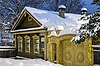
\includegraphics{xeon_files/100px--__.jpg}}\hyperlink{}{
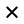
\includegraphics{xeon_files/Close_oojs.png}}
% CentralNotice 


\section{Xeon}[\href{https://ru.wikipedia.org/w/index.php?title=Xeon&amp;veaction=edit&amp;section=0}{править} | \href{https://ru.wikipedia.org/w/index.php?title=Xeon&amp;action=edit&amp;section=0&amp;summary=/*%20%D0%9F%D1%80%D0%B5%D0%B0%D0%BC%D0%B1%D1%83%D0%BB%D0%B0%20*/%20}{править код}]Материал из Википедии — свободной энциклопедииТекущая версия страницы пока \href{https://ru.wikipedia.org/wiki/%D0%92%D0%B8%D0%BA%D0%B8%D0%BF%D0%B5%D0%B4%D0%B8%D1%8F:%D0%9F%D1%80%D0%BE%D0%B2%D0%B5%D1%80%D0%BA%D0%B0_%D1%81%D1%82%D0%B0%D1%82%D0%B5%D0%B9/%D0%9F%D0%BE%D1%8F%D1%81%D0%BD%D0%B5%D0%BD%D0%B8%D0%B5_%D0%B4%D0%BB%D1%8F_%D1%87%D0%B8%D1%82%D0%B0%D1%82%D0%B5%D0%BB%D0%B5%D0%B9}{не проверялась} опытными участниками и может значительно отличаться от \href{https://ru.wikipedia.org/w/index.php?title=Xeon&amp;stable=1}{версии}, проверенной 20 мая 2016; проверки требуют \href{https://ru.wikipedia.org/w/index.php?title=Xeon&amp;oldid=78432884&amp;diff=cur&amp;diffonly=0}{53 правки}.

\includegraphics{xeon_files/1.png}

\includegraphics{xeon_files/arrow-down.png}Текущая версия страницы пока \href{https://ru.wikipedia.org/wiki/%D0%92%D0%B8%D0%BA%D0%B8%D0%BF%D0%B5%D0%B4%D0%B8%D1%8F:%D0%9F%D1%80%D0%BE%D0%B2%D0%B5%D1%80%D0%BA%D0%B0_%D1%81%D1%82%D0%B0%D1%82%D0%B5%D0%B9/%D0%9F%D0%BE%D1%8F%D1%81%D0%BD%D0%B5%D0%BD%D0%B8%D0%B5_%D0%B4%D0%BB%D1%8F_%D1%87%D0%B8%D1%82%D0%B0%D1%82%D0%B5%D0%BB%D0%B5%D0%B9}{не проверялась} опытными участниками и может значительно отличаться от \href{https://ru.wikipedia.org/w/index.php?title=Xeon&amp;stable=1}{версии}, проверенной 20 мая 2016; проверки требуют \href{https://ru.wikipedia.org/w/index.php?title=Xeon&amp;oldid=78432884&amp;diff=cur&amp;diffonly=0}{53 правки}.\hyperlink{mw-head}{Перейти к навигации}\hyperlink{p-search}{Перейти к поиску}
\begin{tabular}\href{https://ru.wikipedia.org/wiki/Pentium_II}{$<$$<$}\nolinebreak\nolinebreak Xeon \nolinebreak\nolinebreak\nolinebreak\nolinebreak
\\\textit{\href{https://ru.wikipedia.org/wiki/%D0%A6%D0%B5%D0%BD%D1%82%D1%80%D0%B0%D0%BB%D1%8C%D0%BD%D1%8B%D0%B9_%D0%BF%D1%80%D0%BE%D1%86%D0%B5%D1%81%D1%81%D0%BE%D1%80}{Центральный процессор}} \\ 
\href{https://ru.wikipedia.org/wiki/%D0%A4%D0%B0%D0%B9%D0%BB:Xeon_new_logo.gif}{
\includegraphics{xeon_files/Xeon_new_logo.gif}}
\\Логотип марки \\ 
\textbf{Производство:} & с апреля 1998 по настоящее время \\ 
\textbf{Производитель:} & \href{https://ru.wikipedia.org/wiki/Intel}{Intel} \\ 
\textbf{Частота \href{https://ru.wikipedia.org/wiki/%D0%A6%D0%B5%D0%BD%D1%82%D1%80%D0%B0%D0%BB%D1%8C%D0%BD%D1%8B%D0%B9_%D0%BF%D1%80%D0%BE%D1%86%D0%B5%D1%81%D1%81%D0%BE%D1%80}{ЦП}:} & 400\nolinebreak\href{https://ru.wikipedia.org/wiki/%D0%9C%D0%93%D1%86}{МГц}\nolinebreak— 4,4\nolinebreak\href{https://ru.wikipedia.org/wiki/%D0%93%D0%93%D1%86}{ГГц} \\ 
\textbf{Частота \href{https://ru.wikipedia.org/wiki/Front_Side_Bus}{FSB}:} & 100\nolinebreak\href{https://ru.wikipedia.org/wiki/%D0%9C%D0%93%D1%86}{МГц}\nolinebreak— 8.0\nolinebreak\href{https://ru.wikipedia.org/wiki/%D0%93%D0%91/%D1%81}{ГБ/с} \\ 
\textbf{Технология производства:} & 250—14\nolinebreak\href{https://ru.wikipedia.org/wiki/%D0%9D%D0%BC}{нм} \\ 
\textbf{\href{https://ru.wikipedia.org/wiki/%D0%A1%D0%B8%D1%81%D1%82%D0%B5%D0%BC%D0%B0_%D0%BA%D0%BE%D0%BC%D0%B0%D0%BD%D0%B4}{Наборы инструкций}:} & \href{https://ru.wikipedia.org/wiki/IA-32}{IA-32}, \href{https://ru.wikipedia.org/wiki/X86-64}{x86-64} \\ 
\textbf{\href{https://ru.wikipedia.org/wiki/%D0%9C%D0%B8%D0%BA%D1%80%D0%BE%D0%B0%D1%80%D1%85%D0%B8%D1%82%D0%B5%D0%BA%D1%82%D1%83%D1%80%D0%B0}{Микроархитектура}:} & \href{https://ru.wikipedia.org/wiki/Intel_P6}{P6}, \href{https://ru.wikipedia.org/wiki/NetBurst}{NetBurst}, \href{https://ru.wikipedia.org/wiki/Intel_Core_(%D0%BC%D0%B8%D0%BA%D1%80%D0%BE%D0%B0%D1%80%D1%85%D0%B8%D1%82%D0%B5%D0%BA%D1%82%D1%83%D1%80%D0%B0)}{Core}, \href{https://ru.wikipedia.org/wiki/Nehalem}{Nehalem}, \href{https://ru.wikipedia.org/wiki/Westmere}{Westmere}, \href{https://ru.wikipedia.org/wiki/Sandy_Bridge}{Sandy Bridge}, \href{https://ru.wikipedia.org/wiki/Broadwell}{Broadwell}, \href{https://ru.wikipedia.org/wiki/Haswell}{Haswell}, \href{https://ru.wikipedia.org/wiki/Skylake}{Skylake} \\ 
\textbf{\href{https://ru.wikipedia.org/wiki/%D0%9C%D0%BD%D0%BE%D0%B3%D0%BE%D1%8F%D0%B4%D0%B5%D1%80%D0%BD%D1%8B%D0%B9_%D0%BF%D1%80%D0%BE%D1%86%D0%B5%D1%81%D1%81%D0%BE%D1%80}{Число ядер}:} & до 72 \\ 
\textbf{\href{https://ru.wikipedia.org/wiki/%D0%A0%D0%B0%D0%B7%D1%8A%D1%91%D0%BC_%D0%BF%D1%80%D0%BE%D1%86%D0%B5%D1%81%D1%81%D0%BE%D1%80%D0%B0_%D0%BF%D0%B5%D1%80%D1%81%D0%BE%D0%BD%D0%B0%D0%BB%D1%8C%D0%BD%D0%BE%D0%B3%D0%BE_%D0%BA%D0%BE%D0%BC%D0%BF%D1%8C%D1%8E%D1%82%D0%B5%D1%80%D0%B0}{Разъёмы}:} & 
\begin{itemize}
	\item \href{https://ru.wikipedia.org/wiki/Slot_2}{Slot 2}
	\item \href{https://ru.wikipedia.org/wiki/Socket_603}{Socket 603}
	\item \href{https://ru.wikipedia.org/wiki/Socket_604}{Socket 604}
	\item \href{https://ru.wikipedia.org/wiki/Socket_J}{Socket J} (LGA 771)
	\item \href{https://ru.wikipedia.org/wiki/Socket_T}{Socket T} (LGA 775)
	\item \href{https://ru.wikipedia.org/wiki/Socket_M}{Socket M} (µPGA 478)
	\item \href{https://ru.wikipedia.org/wiki/Socket_B}{Socket B} (LGA 1366)
	\item \href{https://ru.wikipedia.org/wiki/Socket_H}{Socket H} (LGA 1156)
	\item \href{https://ru.wikipedia.org/wiki/Socket_H2}{Socket H2} (LGA 1155)
	\item \href{https://ru.wikipedia.org/wiki/Socket_LS}{Socket LS} (LGA 1567)
	\item \href{https://ru.wikipedia.org/wiki/Socket_R}{Socket R} (LGA 2011)
	\item \href{https://ru.wikipedia.org/wiki/Socket_H3}{Socket H3} (LGA 1150)
	\item \href{https://ru.wikipedia.org/wiki/LGA_1151}{LGA 1151}
\end{itemize} \\ 
\textbf{\href{https://ru.wikipedia.org/wiki/%D0%AF%D0%B4%D1%80%D0%BE_%D0%BC%D0%B8%D0%BA%D1%80%D0%BE%D0%BF%D1%80%D0%BE%D1%86%D0%B5%D1%81%D1%81%D0%BE%D1%80%D0%B0}{Ядра}:} & 
\begin{itemize}
	\item Drake
	\item Tanner
	\item Cascades
	\item Foster
	\item Prestonia
	\item Gallatin
	\item Nocona, Irwindale, Paxville DP, Dempsey, Harpertown и др.
	\item Gulftown
	\item Beckton
\end{itemize}
\end{tabular}

\textbf{Xeon} — линейка серверных \href{https://ru.wikipedia.org/wiki/%D0%9C%D0%B8%D0%BA%D1%80%D0%BE%D0%BF%D1%80%D0%BE%D1%86%D0%B5%D1%81%D1%81%D0%BE%D1%80}{микропроцессоров} производства \href{https://ru.wikipedia.org/wiki/Intel}{Intel}. Название остаётся неизменным для нескольких поколений \href{https://ru.wikipedia.org/wiki/%D0%A6%D0%B5%D0%BD%D1%82%D1%80%D0%B0%D0%BB%D1%8C%D0%BD%D1%8B%D0%B9_%D0%BF%D1%80%D0%BE%D1%86%D0%B5%D1%81%D1%81%D0%BE%D1%80}{процессоров}. Название ранних моделей состояло из соответствующего названия из ряда настольных \href{https://ru.wikipedia.org/wiki/%D0%A6%D0%B5%D0%BD%D1%82%D1%80%D0%B0%D0%BB%D1%8C%D0%BD%D1%8B%D0%B9_%D0%BF%D1%80%D0%BE%D1%86%D0%B5%D1%81%D1%81%D0%BE%D1%80}{процессоров} и слова Xeon, современные модели имеют в названии только Xeon. В общих чертах серверная линейка процессоров отличается от процессоров для настольных ПК увеличенным объёмом \href{https://ru.wikipedia.org/wiki/%D0%9A%D0%B5%D1%88-%D0%BF%D0%B0%D0%BC%D1%8F%D1%82%D1%8C}{кэш-памяти} и поддержкой многопроцессорных систем большой производительности.

Pentium II Xeon, в отличие от «\href{https://ru.wikipedia.org/wiki/%D0%9D%D0%B0%D1%81%D1%82%D0%BE%D0%BB%D1%8C%D0%BD%D1%8B%D0%B9_%D0%BA%D0%BE%D0%BC%D0%BF%D1%8C%D1%8E%D1%82%D0%B5%D1%80}{десктопного}» \href{https://ru.wikipedia.org/wiki/Pentium_II}{Pentium II}, имел кэш второго уровня, работающий на полной частоте ядра, а не на половине его частоты.

\subsection{Содержание}
\begin{itemize}
	\item \hyperlink{Таблица_микропроцессоров_Xeon}{1Таблица микропроцессоров Xeon}
	\item \hyperlink{Ядро_Nehalem}{2Ядро Nehalem}
\begin{itemize}
	\item \hyperlink{Процессоры_с_индексами_E}{2.1Процессоры с индексами E}
	\item \hyperlink{Процессоры_с_индексами_L}{2.2Процессоры с индексами L}
	\item \hyperlink{Процессоры_с_индексами_W_и_X}{2.3Процессоры с индексами W и X}
\end{itemize}
	\item \hyperlink{Ядро_Westmere}{3Ядро Westmere}
	\item \hyperlink{Ядро_Sandy_Bridge}{4Ядро Sandy Bridge}
	\item \hyperlink{Ядро_Haswell}{5Ядро Haswell}
\begin{itemize}
	\item \hyperlink{E3-12xx_v3-серия_«Haswell»}{5.1E3-12xx v3-серия «Haswell»}
	\item \hyperlink{E5-16xx/26xx_v3-серия_«Haswell-EP»}{5.2E5-16xx/26xx v3-серия «Haswell-EP»}
\end{itemize}
	\item \hyperlink{Ядро_Skylake}{6Ядро Skylake}
\begin{itemize}
	\item \hyperlink{E3-12xx_v5-серия_«Skylake»}{6.1E3-12xx v5-серия «Skylake»}
\end{itemize}
	\item \hyperlink{Серверы_на_базе_Xeon}{7Серверы на базе Xeon}
	\item \hyperlink{Примечания}{8Примечания}
	\item \hyperlink{Ссылки}{9Ссылки}
\end{itemize}

\subsection{Таблица микропроцессоров Xeon[\href{https://ru.wikipedia.org/w/index.php?title=Xeon&amp;veaction=edit&amp;section=1}{править} | \href{https://ru.wikipedia.org/w/index.php?title=Xeon&amp;action=edit&amp;section=1}{править код}]}
\begin{tabular}\textbf{Название} & \textbf{Ядро (кодовое имя)} & \textbf{Частота ядра, МГц} & \textbf{Частота шины / теоретическая пропускная
\\ способность} & \textbf{Кэш} & \textbf{Разъем} & \textbf{Технология, мкм} & \textbf{Напряжение питания, В} & \textbf{Дополнительные возможности} \\ 
Pentium II Xeon & Drake & 400—450 & 100 МГц / 800 МБ/с & L1 16 КБ данных + 16 КБ инструкций;
\\L2 512КБ/1МБ/2МБ & \href{https://ru.wikipedia.org/wiki/Slot_2}{Slot 2} & 0,25 & 2,0 & Поддерживает наборы команд х86 и MMX \\ 
Pentium III Xeon & Tanner & 500—550 & 100 МГц / 800 МБ/с & L1 16 КБ данных + 16 КБ инструкций;
\\L2 512КБ/1МБ/2МБ & Slot 2 & 0,25 & 2,0 & Поддерживает \href{https://ru.wikipedia.org/wiki/SSE}{SSE} и введён серийный номер процессора \\ 
Pentium III Xeon & Cascades & 600—1000 & 133 МГц / 1066 МБ/с & L1 16 КБ данных + 16 КБ инструкций;
\\L2 256 КБ & Slot 2 & 0,18 & 2,8 & Увеличение частоты шины \\ 
Pentium III Xeon & Cascades 2MB & 700—900 & 100 МГц / 800 МБ/с & L1 16 КБ данных + 16 КБ инструкций;
\\L2 2 МБ & Slot 2 & 0,18 & 2,8 & Увеличен кеш второго уровня, поддержка многопроцессорных систем \\ 
Xeon DP & Foster & 1400—2000 & 100 МГц / 3,2 ГБ/с & L1 8 КБ данных + 12 КБ инструкций;
\\L2 256 КБ & \href{https://ru.wikipedia.org/wiki/Socket_603}{Socket 603} & 0,18 & 1,75 & Поддерживает \href{https://ru.wikipedia.org/wiki/SSE2}{SSE2} и убран серийный номер процессора \\ 
Xeon MP & Foster MP & 1400—1600 & 100 МГц / 3,2 Гб/с & L1 8 КБ данных + 12 КБ инструкций;
\\L2 256 КБ;
\\L3 512 КБ / 1 МБ & Socket 603 & 0,18 & 1,75 & Добавлен кеш третьего уровня и поддержка многопроцессорных систем \\ 
LV-Xeon DP & Prestonia & 1600—2800 & 100 МГц / 3,2 ГБ/с & L1 8 КБ данных + 12 КБ инструкций;
\\L2 512 КБ & Socket 603 & 0,13 & 1,3 & Поддержка \href{https://ru.wikipedia.org/wiki/Hyper-Threading}{Hyper-Threading} \\ 
Xeon DP & Prestonia & 2000-3060 & 133 МГц / 4,2 ГБ/с & L1 8 КБ данных + 12 КБ инструкций;
\\L2 512 КБ & \href{https://ru.wikipedia.org/wiki/Socket_604}{Socket 604} & 0,13 & 1,5 & Увеличение частоты шины \\ 
Xeon MP & Gallatin & 3060-3200 & 133 МГц / 4,2 ГБ/с & L1 8 КБ данных + 12 КБ инструкций;
\\L2 512 КБ;
\\L3 1 МБ & Socket 604 & 0,13 & 1,525 & Добавлен кеш третьего уровня \\ 
Xeon MP & Gallatin & 1500-3000 & 100 МГц / 3,2 ГБ/с & L1 8 КБ данных + 12 КБ инструкций;
\\L2 512 КБ;
\\L3 1/2/4 МБ & Socket 603 & 0,13 & 1,525 & Поддержка многопроцессорных систем \\ 
Xeon DP & Nocona & 2800-3600 & 200 МГц / 6,4 ГБ/с & L1 16 КБ данных + 12 КБ инструкций;
\\L2 1 МБ & Socket 604 & 0,09 & 1,325 & Увеличен кэш первого уровня, поддержка \href{https://ru.wikipedia.org/wiki/SSE3}{SSE3}, \href{https://ru.wikipedia.org/wiki/EM64T}{EM64T} и \href{https://ru.wikipedia.org/wiki/NX-%D0%B1%D0%B8%D1%82}{NX-бита} \\ 
Xeon DP & Irwindale & 2800-3800 & 200 МГц / 6,4 ГБ/с & L1 16 КБ данных + 12КБ инструкций;
\\L2 2 МБ & Socket 604 & 0,09 & 1,25-1,388 & Увеличен кэш второго уровня, поддержка \href{https://ru.wikipedia.org/wiki/SSE3}{SSE3}, \href{https://ru.wikipedia.org/wiki/EM64T}{EM64T} и \href{https://ru.wikipedia.org/wiki/NX-%D0%B1%D0%B8%D1%82}{NX-бита} \\ 
Xeon E5 & Haswell-EX & 1600-

3700 & 200 МГц / 6,4 ГБ/с & L1 64 КБ

L2 4608 КБ

L3 46080 КБ & Socket

2011-3 & 0.022 & 1.30В & Увеличен кэш первого, второго уровня, добавлен третий уровень, поддержка MMX, SSE, SSE2, SSE3, SSE4
\end{tabular}

\subsection{Ядро Nehalem[\href{https://ru.wikipedia.org/w/index.php?title=Xeon&amp;veaction=edit&amp;section=2}{править} | \href{https://ru.wikipedia.org/w/index.php?title=Xeon&amp;action=edit&amp;section=2}{править код}]}

Состояние флагманского чипа Intel Xeon, построенного на ядре \href{https://ru.wikipedia.org/wiki/Nehalem}{Nehalem} (на февраль 2010 года).

\subsubsection{Процессоры с индексами E[\href{https://ru.wikipedia.org/w/index.php?title=Xeon&amp;veaction=edit&amp;section=3}{править} | \href{https://ru.wikipedia.org/w/index.php?title=Xeon&amp;action=edit&amp;section=3}{править код}]}
\begin{tabular}\textbf{Название} & \textbf{Intel Xeon Processor E5502$^\hyperlink{cite_note-1}{[1]}$} & \textbf{Intel Xeon Processor E5504$^\hyperlink{cite_note-2}{[2]}$} & \textbf{Intel Xeon Processor E5506$^\hyperlink{cite_note-3}{[3]}$} & \textbf{Intel Xeon Processor E5520$^\hyperlink{cite_note-4}{[4]}$} & \textbf{Intel Xeon Processor E5530$^\hyperlink{cite_note-5}{[5]}$} & \textbf{Intel Xeon Processor E5540$^\hyperlink{cite_note-6}{[6]}$} \\ 
Статус & Производится & Производится & Производится & Производится & Производится & Производится \\ 
Дата начала серийного производства & I кв. 2009 \\ 
Номер процессора & E5502 & E5504 & E5506 & E5520 & E5530 & E5540 \\ 
Количество \href{https://ru.wikipedia.org/wiki/%D0%AF%D0%B4%D1%80%D0%BE_%D0%BC%D0%B8%D0%BA%D1%80%D0%BE%D0%BF%D1%80%D0%BE%D1%86%D0%B5%D1%81%D1%81%D0%BE%D1%80%D0%B0}{ядер} & 2 & 4 \\ 
Количество \href{https://ru.wikipedia.org/wiki/%D0%9C%D0%BD%D0%BE%D0%B3%D0%BE%D0%BF%D0%BE%D1%82%D0%BE%D1%87%D0%BD%D0%BE%D1%81%D1%82%D1%8C}{потоков} & 2 & 4 & 8 \\ 
Базовая \href{https://ru.wikipedia.org/wiki/%D0%A2%D0%B0%D0%BA%D1%82%D0%BE%D0%B2%D0%B0%D1%8F_%D1%87%D0%B0%D1%81%D1%82%D0%BE%D1%82%D0%B0}{тактовая частота} процессора & 1,86 ГГц & 2 ГГц & 2,13 ГГц & 2,26 ГГц & 2,4 ГГц & 2,53 ГГц \\ 
\href{https://ru.wikipedia.org/wiki/%D0%9A%D1%8D%D1%88}{Кэш-память} & 4 МБ «умный» кэш & 8 МБ «умный» кэш \\ 
Тип \href{https://ru.wikipedia.org/wiki/Front_Side_Bus}{шины} & \href{https://ru.wikipedia.org/wiki/Intel_QuickPath_Interconnect}{QPI} \\ 
Производительность системной шины & 4,8 ГТ/сек & 5,86 ГТ/сек \\ 
Количество связей QPI & 2 \\ 
Набор команд & \href{https://ru.wikipedia.org/wiki/IA-64}{64-битный} \\ 
Для встроенного применения? & Нет & Да & Нет & Нет & Нет & Да \\ 
Дополнительный \href{https://ru.wikipedia.org/wiki/SKU}{SKU} & Нет \\ 
Макс. \href{https://ru.wikipedia.org/wiki/TDP}{тепловыделение} & 80 Вт \\ 
Диапазон напряжения питания, VID & 0,75—1,35 В \\ 
Цена (партия\nolinebreak— 1000 шт.) & \$188 & \$224 & \$266 & \$373 & \$530 & \$744 \\ 
\textbf{Спецификация памяти} \\ 
Макс. объём памяти (зависит от типа памяти) & 144 ГБ \\ 
Типы памяти & \href{https://ru.wikipedia.org/wiki/DDR3}{DDR3}-800 & DDR3-800/1066 & DDR3-800/1066 \\ 
Количество каналов памяти & 3 \\ 
Макс. пропускная способность памяти & 19,2 ГБ/сек & 25,6 ГБ/сек \\ 
Расширение физического адреса & 40-битовое \\ 
Поддержка памятью функции \href{https://ru.wikipedia.org/wiki/ECC}{ECC} & Да & Да & Да & Да & Да & Да \\ 
\textbf{Спецификация корпуса} \\ 
Макс. процессоров в конфигурации & 2 \\ 
Температура корпуса &  & 76\nolinebreak°C \\ 
Размер корпуса & 42,5×45 мм \\ 
Норма \href{https://ru.wikipedia.org/wiki/%D0%A4%D0%BE%D1%82%D0%BE%D0%BB%D0%B8%D1%82%D0%BE%D0%B3%D1%80%D0%B0%D1%84%D0%B8%D1%8F}{литографии}\href{https://ru.wikipedia.org/wiki/%D0%A2%D0%B5%D1%85%D0%BF%D1%80%D0%BE%D1%86%D0%B5%D1%81%D1%81}{техпроцесса} & 45 нм \\ 
Размер ядра процессора & 263 мм² \\ 
Количество транзисторов в ядре & 731 млн \\ 
Поддержка \href{https://ru.wikipedia.org/wiki/%D0%A0%D0%B0%D0%B7%D1%8A%D1%91%D0%BC_%D0%BF%D1%80%D0%BE%D1%86%D0%B5%D1%81%D1%81%D0%BE%D1%80%D0%B0_%D0%BF%D0%B5%D1%80%D1%81%D0%BE%D0%BD%D0%B0%D0%BB%D1%8C%D0%BD%D0%BE%D0%B3%D0%BE_%D0%BA%D0%BE%D0%BC%D0%BF%D1%8C%D1%8E%D1%82%D0%B5%D1%80%D0%B0}{процессорного разъёма} & \href{https://ru.wikipedia.org/wiki/Socket_B}{FCLGA1366} \\ 
Без\href{https://ru.wikipedia.org/wiki/%D0%93%D0%B0%D0%BB%D0%BE%D0%B3%D0%B5%D0%BD%D1%8B}{галогенная} продукция? & Да \\ 
\textbf{Применяемые технологии} \\ 
\href{https://ru.wikipedia.org/wiki/Turbo_Boost}{Turbo Boost} & Нет & Да \\ 
\href{https://ru.wikipedia.org/wiki/Hyper-Threading}{Hyper-Threading} & Нет & Нет & Нет & Да & Да & Да \\ 
\href{https://ru.wikipedia.org/wiki/%D0%92%D0%B8%D1%80%D1%82%D1%83%D0%B0%D0%BB%D0%B8%D0%B7%D0%B0%D1%86%D0%B8%D1%8F}{Виртуализация} (VT-x) & Да \\ 
Виртуализации прямого ввода-вывода (\href{https://ru.wikipedia.org/wiki/VT-d}{VT-d}) & Да \\ 
\href{https://ru.wikipedia.org/wiki/%D0%94%D0%BE%D0%B2%D0%B5%D1%80%D0%B5%D0%BD%D0%BD%D0%B0%D1%8F_%D0%B7%D0%B0%D0%B3%D1%80%D1%83%D0%B7%D0%BA%D0%B0_(%D0%B0%D0%BF%D0%BF%D0%B0%D1%80%D0%B0%D1%82%D0%BD%D1%8B%D0%B5_%D1%81%D1%80%D0%B5%D0%B4%D1%81%D1%82%D0%B2%D0%B0)#Intel_Trusted_Execution_Technology}{Trusted Execution} & Нет \\ 
Новые AES инструкции &  \\ 
Intel 64 & Да \\ 
Idle States & Да \\ 
Улучшенная технология \href{https://ru.wikipedia.org/wiki/SpeedStep}{SpeedStep} & Да \\ 
Demand Based Switching & Да \\ 
\href{https://ru.wikipedia.org/wiki/NX-%D0%B1%D0%B8%D1%82}{Execute Disable Bit} & Да
\end{tabular}

\subsubsection{Процессоры с индексами L[\href{https://ru.wikipedia.org/w/index.php?title=Xeon&amp;veaction=edit&amp;section=4}{править} | \href{https://ru.wikipedia.org/w/index.php?title=Xeon&amp;action=edit&amp;section=4}{править код}]}
\begin{tabular}\textbf{Название} & \textbf{Intel Xeon Processor L5506$^\hyperlink{cite_note-7}{[7]}$} & \textbf{Intel Xeon Processor L5508$^\hyperlink{cite_note-8}{[8]}$} & \textbf{Intel Xeon Processor L5518$^\hyperlink{cite_note-9}{[9]}$} & \textbf{Intel Xeon Processor L5520$^\hyperlink{cite_note-10}{[10]}$} & \textbf{Intel Xeon Processor L5530$^\hyperlink{cite_note-11}{[11]}$} \\ 
Статус & Производится & Производится & Производится & Производится & Производится \\ 
Дата начала серийного производства & I кв. 2009 & III кв. 2009 \\ 
Номер процессора & L5506 & L5508 & L5518 & L5520 & L5530 \\ 
Количество \href{https://ru.wikipedia.org/wiki/%D0%AF%D0%B4%D1%80%D0%BE_%D0%BC%D0%B8%D0%BA%D1%80%D0%BE%D0%BF%D1%80%D0%BE%D1%86%D0%B5%D1%81%D1%81%D0%BE%D1%80%D0%B0}{ядер} & 4 & 2 & 4 \\ 
Количество \href{https://ru.wikipedia.org/wiki/%D0%9C%D0%BD%D0%BE%D0%B3%D0%BE%D0%BF%D0%BE%D1%82%D0%BE%D1%87%D0%BD%D0%BE%D1%81%D1%82%D1%8C}{потоков} & 4 & 8 \\ 
Базовая \href{https://ru.wikipedia.org/wiki/%D0%A2%D0%B0%D0%BA%D1%82%D0%BE%D0%B2%D0%B0%D1%8F_%D1%87%D0%B0%D1%81%D1%82%D0%BE%D1%82%D0%B0}{тактовая частота} процессора & 2,13 ГГц & 2 ГГц & 2,13 ГГц & 2,26 ГГц & 2,4 ГГц \\ 
\href{https://ru.wikipedia.org/wiki/%D0%9A%D1%8D%D1%88}{Кэш-память} & 4 МБ «умный» кэш & 8 МБ «умный» кэш \\ 
Тип \href{https://ru.wikipedia.org/wiki/Front_Side_Bus}{шины} & \href{https://ru.wikipedia.org/wiki/Intel_QuickPath_Interconnect}{QPI} \\ 
Производительность системной шины & 4,8 ГТ/сек & 5,86 ГТ/сек \\ 
Количество связей QPI & 2 \\ 
Набор команд & \href{https://ru.wikipedia.org/wiki/IA-64}{64-битный} \\ 
Для встроенного применения? & Нет & Да & Да & Нет & Нет \\ 
Дополнительный \href{https://ru.wikipedia.org/wiki/SKU}{SKU} & Нет \\ 
Макс. \href{https://ru.wikipedia.org/wiki/TDP}{тепловыделение} & 60 Вт & 38 Вт & 60 Вт \\ 
Диапазон напряжения питания, VID & 0,75—1,35 В \\ 
Цена (партия\nolinebreak— 1000 шт.) & \$423 \\ 
\$530 & \$744 \\ 
\textbf{Спецификация памяти} \\ 
Макс. объём памяти (зависит от типа памяти) & 144 ГБ \\ 
Типы памяти & DDR3-800 & DDR3-800/1066 \\ 
Количество каналов памяти & 3 \\ 
Макс. пропускная способность памяти & 19,2 ГБ/сек & 25,6 ГБ/сек \\ 
Расширение физического адреса & 40-битовое \\ 
Поддержка памятью функции \href{https://ru.wikipedia.org/wiki/ECC}{ECC} & Да & Да & Да & Да & Да \\ 
\textbf{Спецификация корпуса} \\ 
Макс. процессоров в конфигурации & 2 \\ 
Температура корпуса & 70\nolinebreak°C & 85\nolinebreak°C & 85\nolinebreak°C & 70\nolinebreak°C &  \\ 
Размер корпуса & 42,5×45 мм \\ 
Норма \href{https://ru.wikipedia.org/wiki/%D0%A4%D0%BE%D1%82%D0%BE%D0%BB%D0%B8%D1%82%D0%BE%D0%B3%D1%80%D0%B0%D1%84%D0%B8%D1%8F}{литографии}\href{https://ru.wikipedia.org/wiki/%D0%A2%D0%B5%D1%85%D0%BF%D1%80%D0%BE%D1%86%D0%B5%D1%81%D1%81}{техпроцесса} & 45 нм \\ 
Размер ядра процессора & 263 мм² \\ 
Количество транзисторов в ядре & 731\nolinebreakмлн. \\ 
Поддержка \href{https://ru.wikipedia.org/wiki/%D0%A0%D0%B0%D0%B7%D1%8A%D1%91%D0%BC_%D0%BF%D1%80%D0%BE%D1%86%D0%B5%D1%81%D1%81%D0%BE%D1%80%D0%B0_%D0%BF%D0%B5%D1%80%D1%81%D0%BE%D0%BD%D0%B0%D0%BB%D1%8C%D0%BD%D0%BE%D0%B3%D0%BE_%D0%BA%D0%BE%D0%BC%D0%BF%D1%8C%D1%8E%D1%82%D0%B5%D1%80%D0%B0}{процессорного разъёма} & \href{https://ru.wikipedia.org/wiki/Socket_B}{FCLGA1366} \\ 
Без\href{https://ru.wikipedia.org/wiki/%D0%93%D0%B0%D0%BB%D0%BE%D0%B3%D0%B5%D0%BD%D1%8B}{галогенная} продукция? & Да \\ 
\textbf{Применение новых технологий} \\ 
\href{https://ru.wikipedia.org/wiki/Turbo_Boost}{Turbo Boost} & Нет & Да \\ 
\href{https://ru.wikipedia.org/wiki/Hyper-Threading}{Hyper-Threading} & Нет & Да & Да & Да & Да \\ 
\href{https://ru.wikipedia.org/wiki/%D0%92%D0%B8%D1%80%D1%82%D1%83%D0%B0%D0%BB%D0%B8%D0%B7%D0%B0%D1%86%D0%B8%D1%8F}{Виртуализация} (VT-x) & Да \\ 
Виртуализация прямого ввода-вывода (\href{https://ru.wikipedia.org/wiki/VT-d}{VT-d}) & Да \\ 
\href{https://ru.wikipedia.org/wiki/%D0%94%D0%BE%D0%B2%D0%B5%D1%80%D0%B5%D0%BD%D0%BD%D0%B0%D1%8F_%D0%B7%D0%B0%D0%B3%D1%80%D1%83%D0%B7%D0%BA%D0%B0_(%D0%B0%D0%BF%D0%BF%D0%B0%D1%80%D0%B0%D1%82%D0%BD%D1%8B%D0%B5_%D1%81%D1%80%D0%B5%D0%B4%D1%81%D1%82%D0%B2%D0%B0)#Intel_Trusted_Execution_Technology}{Trusted Execution} & Нет \\ 
Новые AES инструкции &  & Нет \\ 
Intel 64 & Да \\ 
Idle States & Да \\ 
Улучшенная технология \href{https://ru.wikipedia.org/wiki/SpeedStep}{SpeedStep} & Да \\ 
Demand Based Switching & Да \\ 
\href{https://ru.wikipedia.org/wiki/NX-%D0%B1%D0%B8%D1%82}{Execute Disable Bit} & Да
\end{tabular}

\subsubsection{Процессоры с индексами W и X[\href{https://ru.wikipedia.org/w/index.php?title=Xeon&amp;veaction=edit&amp;section=5}{править} | \href{https://ru.wikipedia.org/w/index.php?title=Xeon&amp;action=edit&amp;section=5}{править код}]}
\begin{tabular}\textbf{Название} & \textbf{Intel Xeon Processor W5580$^\hyperlink{cite_note-12}{[12]}$} & \textbf{Intel Xeon Processor W5590$^\hyperlink{cite_note-13}{[13]}$} & \textbf{Intel Xeon Processor X5550$^\hyperlink{cite_note-14}{[14]}$} & \textbf{Intel Xeon Processor X5560$^\hyperlink{cite_note-15}{[15]}$} & \textbf{Intel Xeon Processor X5570$^\hyperlink{cite_note-16}{[16]}$} \\ 
Статус & Производится & Производится & Производится & Производится & Производится \\ 
Дата начала серийного производства & I кв. 2009 & III кв. 2009 & I кв. 2009 \\ 
Номер процессора & W5580 & W5590 & X5550 & X5560 & X5570 \\ 
Количество \href{https://ru.wikipedia.org/wiki/%D0%AF%D0%B4%D1%80%D0%BE_%D0%BC%D0%B8%D0%BA%D1%80%D0%BE%D0%BF%D1%80%D0%BE%D1%86%D0%B5%D1%81%D1%81%D0%BE%D1%80%D0%B0}{ядер} & 4 \\ 
Количество \href{https://ru.wikipedia.org/wiki/%D0%9C%D0%BD%D0%BE%D0%B3%D0%BE%D0%BF%D0%BE%D1%82%D0%BE%D1%87%D0%BD%D0%BE%D1%81%D1%82%D1%8C}{потоков} & 8 \\ 
Базовая \href{https://ru.wikipedia.org/wiki/%D0%A2%D0%B0%D0%BA%D1%82%D0%BE%D0%B2%D0%B0%D1%8F_%D1%87%D0%B0%D1%81%D1%82%D0%BE%D1%82%D0%B0}{тактовая частота} процессора & 3,2 ГГц & 3,33 ГГц & 2,66 ГГц & 2,8 ГГц & 2,93 ГГц \\ 
\href{https://ru.wikipedia.org/wiki/%D0%9A%D1%8D%D1%88}{Кэш-память} & 8 МБ «умный» кэш \\ 
Тип \href{https://ru.wikipedia.org/wiki/Front_Side_Bus}{шины} & \href{https://ru.wikipedia.org/wiki/Intel_QuickPath_Interconnect}{QPI} \\ 
Производительность системной шины & 6,4 ГТ/сек \\ 
Количество связей QPI & 2 \\ 
Набор команд & \href{https://ru.wikipedia.org/wiki/IA-64}{64-битный} \\ 
Для встроенного применения? & Нет & Нет & Нет & Нет & Нет \\ 
Дополнительный \href{https://ru.wikipedia.org/wiki/SKU}{SKU} & Нет \\ 
Макс. \href{https://ru.wikipedia.org/wiki/TDP}{тепловыделение} & 130 Вт & 95 Вт \\ 
Диапазон напряжения питания, VID & 0,75—1,35 В \\ 
Цена (партия\nolinebreak— 1000 шт.) & \$1600 & \$1600 & \$958 & \$1172 & \$1386 \\ 
\textbf{Спецификация памяти} \\ 
Макс. объём памяти (зависит от типа памяти) & 144 ГБ \\ 
Типы памяти & DDR3-800/1066/1333 & Н/Д & DDR3-800/1066/1333 \\ 
Количество каналов памяти & 3 \\ 
Макс. пропускная способность памяти & 32 ГБ/сек & Н/Д & 32 ГБ/сек \\ 
Расширение физического адреса & 40-битовое \\ 
Поддержка памятью функции \href{https://ru.wikipedia.org/wiki/ECC}{ECC} & Да & Да$^\hyperlink{cite_note-17}{[17]}$ & Да & Да & Да \\ 
\textbf{Спецификация корпуса} \\ 
Макс. процессоров в конфигурации & 2 \\ 
Температура корпуса &  & 75\nolinebreak°C \\ 
Размер корпуса & 42,5×45 мм \\ 
Норма \href{https://ru.wikipedia.org/wiki/%D0%A4%D0%BE%D1%82%D0%BE%D0%BB%D0%B8%D1%82%D0%BE%D0%B3%D1%80%D0%B0%D1%84%D0%B8%D1%8F}{литографии}\href{https://ru.wikipedia.org/wiki/%D0%A2%D0%B5%D1%85%D0%BF%D1%80%D0%BE%D1%86%D0%B5%D1%81%D1%81}{техпроцесса} & 45 нм \\ 
Размер ядра процессора & 263 мм² \\ 
Количество транзисторов в ядре & 731 млн \\ 
Поддержка \href{https://ru.wikipedia.org/wiki/%D0%A0%D0%B0%D0%B7%D1%8A%D1%91%D0%BC_%D0%BF%D1%80%D0%BE%D1%86%D0%B5%D1%81%D1%81%D0%BE%D1%80%D0%B0_%D0%BF%D0%B5%D1%80%D1%81%D0%BE%D0%BD%D0%B0%D0%BB%D1%8C%D0%BD%D0%BE%D0%B3%D0%BE_%D0%BA%D0%BE%D0%BC%D0%BF%D1%8C%D1%8E%D1%82%D0%B5%D1%80%D0%B0}{процессорного разъёма} & \href{https://ru.wikipedia.org/wiki/Socket_B}{FCLGA1366} \\ 
Без\href{https://ru.wikipedia.org/wiki/%D0%93%D0%B0%D0%BB%D0%BE%D0%B3%D0%B5%D0%BD%D1%8B}{галогенная} продукция? & Да \\ 
\textbf{Применение новых технологий} \\ 
\href{https://ru.wikipedia.org/wiki/Turbo_Boost}{Turbo Boost} & Да \\ 
\href{https://ru.wikipedia.org/wiki/Hyper-Threading}{Hyper-Threading} & Да & Да & Да & Да & Да \\ 
\href{https://ru.wikipedia.org/wiki/%D0%92%D0%B8%D1%80%D1%82%D1%83%D0%B0%D0%BB%D0%B8%D0%B7%D0%B0%D1%86%D0%B8%D1%8F}{Виртуализация} (VT-x) & Да \\ 
Виртуализация прямого ввода-вывода (\href{https://ru.wikipedia.org/wiki/VT-d}{VT-d}) & Да \\ 
\href{https://ru.wikipedia.org/wiki/%D0%94%D0%BE%D0%B2%D0%B5%D1%80%D0%B5%D0%BD%D0%BD%D0%B0%D1%8F_%D0%B7%D0%B0%D0%B3%D1%80%D1%83%D0%B7%D0%BA%D0%B0_(%D0%B0%D0%BF%D0%BF%D0%B0%D1%80%D0%B0%D1%82%D0%BD%D1%8B%D0%B5_%D1%81%D1%80%D0%B5%D0%B4%D1%81%D1%82%D0%B2%D0%B0)#Intel_Trusted_Execution_Technology}{Trusted Execution} & Нет \\ 
Новые AES инструкции & Нет & Нет &  \\ 
Intel 64 & Да \\ 
Idle States & Да \\ 
Улучшенная технология \href{https://ru.wikipedia.org/wiki/SpeedStep}{SpeedStep} & Да \\ 
Demand Based Switching & Да \\ 
\href{https://ru.wikipedia.org/wiki/NX-%D0%B1%D0%B8%D1%82}{Execute Disable Bit} & Да
\end{tabular}

\subsection{Ядро Westmere[\href{https://ru.wikipedia.org/w/index.php?title=Xeon&amp;veaction=edit&amp;section=6}{править} | \href{https://ru.wikipedia.org/w/index.php?title=Xeon&amp;action=edit&amp;section=6}{править код}]}

В \href{https://ru.wikipedia.org/wiki/%D0%9C%D0%B0%D1%80%D1%82}{марте}\href{https://ru.wikipedia.org/wiki/2010_%D0%B3%D0%BE%D0%B4}{2010 года} Intel представила 8-ядерные процессоры семейства Intel Xeon 7500 с ядрами новой архитектуры \href{https://ru.wikipedia.org/wiki/Westmere}{Westmere}$^\hyperlink{cite_note-18}{[18]}$.

В \href{https://ru.wikipedia.org/wiki/%D0%90%D0%BF%D1%80%D0%B5%D0%BB%D1%8C}{апреле}\href{https://ru.wikipedia.org/wiki/2011_%D0%B3%D0%BE%D0%B4}{2011 года} Intel представила очередные процессоры под маркой Xeon$^\hyperlink{cite_note-3dnews-1-19}{[19]}$, имеющие технологический процесс 32 нм и разъём LGA 1155:
\begin{itemize}
	\item Intel Xeon E3-1290\nolinebreak— 3,6 ГГц (до 4,0 ГГц), 4 ядра, 8 потоков, кэш L2=1 МБ, кэш L3=8 МБ, TDP 95 Вт
	\item Intel Xeon E3-1280\nolinebreak— 3,5 ГГц (до 3,9 ГГц), 4 ядра, 8 потоков, кэш L2=1 МБ, кэш L3=8 МБ, TDP 95 Вт
	\item Intel Xeon E3-1275\nolinebreak— 3,4 ГГц (до 3,8 ГГц), 4 ядра, 8 потоков, кэш L2=1 МБ, кэш L3=8 МБ, TDP 95 Вт, Intel HD Graphics P3000
	\item Intel Xeon E3-1270\nolinebreak— 3,4 ГГц (до 3,8 ГГц), 4 ядра, 8 потоков, кэш L2=1 МБ, кэш L3=8 МБ, TDP 80 Вт
	\item Intel Xeon E3-1260L\nolinebreak— 2,4 ГГц (до 3,3 ГГц), 4 ядра, 8 потоков, кэш L2=1 МБ, кэш L3=8 МБ, TDP 45 Вт, Intel HD Graphics P2000
	\item Intel Xeon E3-1245\nolinebreak— 3,3 ГГц (до 3,7 ГГц), 4 ядра, 8 потоков, кэш L2=1 МБ, кэш L3=8 МБ, TDP 95 Вт, Intel HD Graphics P3000
	\item Intel Xeon E3-1240\nolinebreak— 3,3 ГГц (до 3,7 ГГц), 4 ядра, 8 потоков, кэш L2=1 МБ, кэш L3=8 МБ, TDP 80 Вт
	\item Intel Xeon E3-1235\nolinebreak— 3,2 ГГц (до 3,6 ГГц), 4 ядра, 8 потоков, кэш L2=1 МБ, кэш L3=8 МБ, TDP 95 Вт, Intel HD Graphics P3000
	\item Intel Xeon E3-1230\nolinebreak— 3,2 ГГц (до 3,6 ГГц), 4 ядра, 8 потоков, кэш L2=1 МБ, кэш L3=8 МБ, TDP 80 Вт
	\item Intel Xeon E3-1231\nolinebreak— 3,4 ГГц (до 3,8 ГГц), 4 ядра, 8 потоков, кэш L2=1 МБ, кэш L3=8 МБ, TDP 80 Вт
	\item Intel Xeon E3-1225\nolinebreak— 3,1 ГГц (до 3,4 ГГц), 4 ядра, 4 потока, кэш L2=1 МБ, кэш L3=6 МБ, TDP 95 Вт, Intel HD Graphics P3000
	\item Intel Xeon E3-1220L\nolinebreak— 2,2 ГГц (до 3,4 ГГц), 2 ядра, 4 потока, кэш L2=512 КБ, кэш L3=3 МБ, TDP 20 Вт
	\item Intel Xeon E3-1220\nolinebreak— 3,1 ГГц (до 3,4 ГГц), 4 ядра, 4 потока, кэш L2=1 МБ, кэш L3=8 МБ, TDP 80 Вт
\end{itemize}

\subsection{Ядро Sandy Bridge[\href{https://ru.wikipedia.org/w/index.php?title=Xeon&amp;veaction=edit&amp;section=7}{править} | \href{https://ru.wikipedia.org/w/index.php?title=Xeon&amp;action=edit&amp;section=7}{править код}]}

В конце \href{https://ru.wikipedia.org/wiki/2011_%D0%B3%D0%BE%D0%B4}{2011 года} Intel начала тестирование процессоров Xeon E5 основанных на новой \href{https://ru.wikipedia.org/wiki/%D0%9C%D0%B8%D0%BA%D1%80%D0%BE%D0%B0%D1%80%D1%85%D0%B8%D1%82%D0%B5%D0%BA%D1%82%D1%83%D1%80%D0%B0}{микроархитектуре}\href{https://ru.wikipedia.org/wiki/Sandy_Bridge}{Sandy Bridge}$^\hyperlink{cite_note-3dnews-2-20}{[20]}$.

\subsection{Ядро Haswell[\href{https://ru.wikipedia.org/w/index.php?title=Xeon&amp;veaction=edit&amp;section=8}{править} | \href{https://ru.wikipedia.org/w/index.php?title=Xeon&amp;action=edit&amp;section=8}{править код}]}

\subsubsection{E3-12xx v3-серия «Haswell»[\href{https://ru.wikipedia.org/w/index.php?title=Xeon&amp;veaction=edit&amp;section=9}{править} | \href{https://ru.wikipedia.org/w/index.php?title=Xeon&amp;action=edit&amp;section=9}{править код}]}

Представленный в мае 2013 года Xeon E3-12xx v3 стал первым представителем Xeon серии на микроархитектуре \href{https://ru.wikipedia.org/wiki/Haswell}{Haswell}. Разработан под разъём \href{https://ru.wikipedia.org/wiki/LGA_1150}{LGA 1150}, представленный ранее для десктопной серии Core i5/i7 Haswell-процессоров. Как и ранее, основное отличие между десктоп- и серверной версией процессора является поддержка \href{https://ru.wikipedia.org/wiki/ECC}{ECC}-памяти. Основное преимущество новой микроархитектуры\nolinebreak— улучшенная энергоэффективность. Следуя принятой маркировке, Xeon E5-26xx v3 серия позволяет создавать многопроцессорные сервера.

\subsubsection{E5-16xx/26xx v3-серия «Haswell-EP»[\href{https://ru.wikipedia.org/w/index.php?title=Xeon&amp;veaction=edit&amp;section=10}{править} | \href{https://ru.wikipedia.org/w/index.php?title=Xeon&amp;action=edit&amp;section=10}{править код}]}

Представленные в сентябре 2014 Xeon E5-16xx v3 и Xeon E5-26xx v3 процессоры используют новый разъём LGA 2011-v3, несовместимый с \href{https://ru.wikipedia.org/wiki/LGA_2011}{LGA 2011} (совместим только при скальпировании процессора), использовавшейся ранее в микроархитектурах Sandy Bridge и Ivy Bridge. Основное преимущество этого поколения\nolinebreak— улучшенная энергоэффективность, больше ядер и увеличенные кэши последнего уровня (\href{https://ru.wikipedia.org/wiki/%D0%90%D0%BD%D0%B3%D0%BB%D0%B8%D0%B9%D1%81%D0%BA%D0%B8%D0%B9_%D1%8F%D0%B7%D1%8B%D0%BA}{англ.}\nolinebreaklast level cache, LLC).

\subsection{Ядро Skylake[\href{https://ru.wikipedia.org/w/index.php?title=Xeon&amp;veaction=edit&amp;section=11}{править} | \href{https://ru.wikipedia.org/w/index.php?title=Xeon&amp;action=edit&amp;section=11}{править код}]}

\subsubsection{E3-12xx v5-серия «Skylake»[\href{https://ru.wikipedia.org/w/index.php?title=Xeon&amp;veaction=edit&amp;section=12}{править} | \href{https://ru.wikipedia.org/w/index.php?title=Xeon&amp;action=edit&amp;section=12}{править код}]}

В конце 2015 года Intel представила очередную линейку процессоров Xeon с разъемом LGA1151 для серверов начального уровня, процессоры привычно стали полным аналогом десктопных Core i7 6-го поколения, но, в отличие от предыдущих поколений Xeon для разъемов \href{https://ru.wikipedia.org/wiki/Lga1150}{LGA1150} и \href{https://ru.wikipedia.org/wiki/LGA1155}{LGA1155}, Intel полностью заблокировала работоспособность данных процессоров в «обычных» (десктопных) материнских платах с чипсетами H110, B150, Z170 и других. Для функционирования Xeon E3-12xx V5 обязательно требуется материнская плата с чипсетами C232 или C236.

\subsection{Серверы на базе Xeon[\href{https://ru.wikipedia.org/w/index.php?title=Xeon&amp;veaction=edit&amp;section=13}{править} | \href{https://ru.wikipedia.org/w/index.php?title=Xeon&amp;action=edit&amp;section=13}{править код}]}

Процессоры Intel Xeon используются в серверах \href{https://ru.wikipedia.org/wiki/IBM}{IBM}, \href{https://ru.wikipedia.org/wiki/Dell}{Dell}, \href{https://ru.wikipedia.org/wiki/Hewlett-Packard}{Hewlett-Packard}, \href{https://ru.wikipedia.org/wiki/Sun_Microsystems}{Sun Microsystems}, \href{https://ru.wikipedia.org/wiki/Fujitsu}{Fujitsu} и других производителей.

\subsection{Примечания[\href{https://ru.wikipedia.org/w/index.php?title=Xeon&amp;veaction=edit&amp;section=14}{править} | \href{https://ru.wikipedia.org/w/index.php?title=Xeon&amp;action=edit&amp;section=14}{править код}]}
\begin{enumerate}
	\item \hyperlink{cite_ref-1}{Перейти ↑}\href{http://ark.intel.com/Product.aspx?id=37092}{Intel Xeon Processor E5502 (4M Cache, 1.86 GHz, 4.80 GT/s Intel QPI)}\nolinebreak(англ.)
	\item \hyperlink{cite_ref-2}{Перейти ↑}\href{http://ark.intel.com/Product.aspx?id=37092}{Intel Xeon Processor E5504 (4M Cache, 2.00 GHz, 4.80 GT/s Intel QPI)}\nolinebreak(англ.)
	\item \hyperlink{cite_ref-3}{Перейти ↑}\href{http://ark.intel.com/Product.aspx?id=37092}{Intel Xeon Processor E5506(4M Cache, 2.13 GHz, 4.80 GT/s Intel QPI)}\nolinebreak(англ.)
	\item \hyperlink{cite_ref-4}{Перейти ↑}\href{http://ark.intel.com/Product.aspx?id=37092}{Intel Xeon Processor E5520 (8M Cache, 2.26 GHz, 5.86 GT/s Intel QPI)}\nolinebreak(англ.)
	\item \hyperlink{cite_ref-5}{Перейти ↑}\href{http://ark.intel.com/Product.aspx?id=37103}{Intel Xeon Processor E5530 (8M Cache, 2.40 GHz, 5.86 GT/s Intel QPI)}\nolinebreak(англ.)
	\item \hyperlink{cite_ref-6}{Перейти ↑}\href{http://ark.intel.com/Product.aspx?id=37104}{Intel Xeon Processor E5540 (8M Cache, 2.53 GHz, 5.86 GT/s Intel QPI)}\nolinebreak(англ.)
	\item \hyperlink{cite_ref-7}{Перейти ↑}\href{http://ark.intel.com/Product.aspx?id=40712}{Intel Xeon Processor L5506 (4M Cache, 2.13 GHz, 4.80 GT/s Intel QPI)}\nolinebreak(англ.)
	\item \hyperlink{cite_ref-8}{Перейти ↑}\href{http://ark.intel.com/Product.aspx?id=40726}{Intel Xeon Processor L5508 (8M Cache, 2.00 GHz, 5.86 GT/s Intel QPI)}\nolinebreak(англ.)
	\item \hyperlink{cite_ref-9}{Перейти ↑}\href{http://ark.intel.com/Product.aspx?id=40727}{Intel Xeon Processor L5518 (8M Cache, 2.13 GHz, 5.86 GT/s Intel QPI)}\nolinebreak(англ.)
	\item \hyperlink{cite_ref-10}{Перейти ↑}\href{http://ark.intel.com/Product.aspx?id=40727}{Intel Xeon Processor L5520 (8M Cache, 2.26 GHz, 5.86 GT/s Intel QPI)}\nolinebreak(англ.)
	\item \hyperlink{cite_ref-11}{Перейти ↑}\href{http://ark.intel.com/Product.aspx?id=41755}{Intel Xeon Processor L5530 (8M Cache, 2.40 GHz, 5.86 GT/s Intel QPI)}\nolinebreak(англ.)
	\item \hyperlink{cite_ref-12}{Перейти ↑}\href{http://ark.intel.com/Product.aspx?id=37113}{Intel Xeon Processor W5580 (8M Cache, 3.20 GHz, 6.40 GT/s Intel QPI)}\nolinebreak(англ.)
	\item \hyperlink{cite_ref-13}{Перейти ↑}\href{http://ark.intel.com/Product.aspx?id=41643}{Intel Xeon Processor W5590 (8M Cache, 3.33 GHz, 6.40 GT/s Intel QPI)}\nolinebreak(англ.)
	\item \hyperlink{cite_ref-14}{Перейти ↑}\href{http://ark.intel.com/Product.aspx?id=37106}{Intel Xeon Processor X5550 (8M Cache, 2.66 GHz, 6.40 GT/s Intel QPI)}\nolinebreak(англ.)
	\item \hyperlink{cite_ref-15}{Перейти ↑}\href{http://ark.intel.com/Product.aspx?id=37109}{Intel Xeon Processor X5560 (8M Cache, 2.80 GHz, 6.40 GT/s Intel QPI)}\nolinebreak(англ.)
	\item \hyperlink{cite_ref-16}{Перейти ↑}\href{http://ark.intel.com/Product.aspx?id=37111}{Intel Xeon Processor X5570 (8M Cache, 2.93 GHz, 6.40 GT/s Intel QPI)}\nolinebreak(англ.)
	\item \hyperlink{cite_ref-17}{Перейти ↑}\href{http://ark.intel.com/products/41643/Intel-Xeon-Processor-W5590-8M-Cache-3_33-GHz-6_40-GTs-Intel-QPI}{Intel Xeon Processor W5590 (8M Cache, 3.33 GHz, 6.40 GT/s Intel QPI) Specifications}.  Intel ARK (Product Specs). \scriptsize Проверено 21 апреля 2016. \normalsize
	\item \hyperlink{cite_ref-18}{Перейти ↑}\href{http://www.3dnews.ru/news/ofitsialnii_reliz_intel_xeon_7500_series}{Официальный релиз Intel Xeon 7500 Series}. // \href{https://ru.wikipedia.org/wiki/3DNews}{3DNews}.
	\item \hyperlink{cite_ref-3dnews-1_19-0}{Перейти ↑}\href{http://www.3dnews.ru/news/609624}{Intel представила в России новые процессоры Xeon серий E7 и E3-1200}. // \href{https://ru.wikipedia.org/wiki/3DNews}{3DNews}. 15.04.2011.
	\item \hyperlink{cite_ref-3dnews-2_20-0}{Перейти ↑}\href{http://www.3dnews.ru/news/620530}{Показатели производительности серверных 8-ядерных Sandy Bridge-EP}. // \href{https://ru.wikipedia.org/wiki/3DNews}{3DNews}. 29.11.2011.
\end{enumerate}

\subsection{Ссылки[\href{https://ru.wikipedia.org/w/index.php?title=Xeon&amp;veaction=edit&amp;section=15}{править} | \href{https://ru.wikipedia.org/w/index.php?title=Xeon&amp;action=edit&amp;section=15}{править код}]}
\begin{itemize}
	\item \href{http://www.intel.com/ru_RU/products/server/processor/}{Серверные процессоры Xeon}
	\item \href{http://www.intel.com/support/ru/processors/xeon/index.htm}{Процессор Intel Xeon}
\end{itemize}
\begin{tabular}\textbf{[\href{javascript:collapseTable(0);}{показать}]\href{https://ru.wikipedia.org/wiki/%D0%A8%D0%B0%D0%B1%D0%BB%D0%BE%D0%BD:%D0%9F%D1%80%D0%BE%D1%86%D0%B5%D1%81%D1%81%D0%BE%D1%80%D1%8B_Intel}{

\includegraphics{xeon_files/14px-Wikipedia_interwiki_section_gear_icon.png}}\href{https://ru.wikipedia.org/wiki/%D0%A1%D0%BF%D0%B8%D1%81%D0%BE%D0%BA_%D0%BC%D0%B8%D0%BA%D1%80%D0%BE%D0%BF%D1%80%D0%BE%D1%86%D0%B5%D1%81%D1%81%D0%BE%D1%80%D0%BE%D0%B2_Intel}{Процессоры Intel}} \\ 

\begin{tabular} \\ 
 & \textbf{Больше не
\\производятся} & 
\begin{tabular} \\ 
 & \textbf{Разрядность 4 бита:} & 
\begin{itemize}
	\item \href{https://ru.wikipedia.org/wiki/4004}{4004}
	\item \href{https://ru.wikipedia.org/wiki/4040}{4040}
\end{itemize} \\ 
\textbf{Разрядность \href{https://ru.wikipedia.org/wiki/8_%D0%B1%D0%B8%D1%82_(%D0%BA%D0%BE%D0%BC%D0%BF%D1%8C%D1%8E%D1%82%D0%B5%D1%80%D0%BD%D0%B0%D1%8F_%D0%B0%D1%80%D1%85%D0%B8%D1%82%D0%B5%D0%BA%D1%82%D1%83%D1%80%D0%B0)}{8 бит}:} & 
\begin{itemize}
	\item \href{https://ru.wikipedia.org/wiki/8008}{8008}
	\item \href{https://ru.wikipedia.org/wiki/8080}{8080}
	\item \href{https://ru.wikipedia.org/wiki/8085}{8085}
\end{itemize} \\ 
\textbf{Разрядность \href{https://ru.wikipedia.org/wiki/16_%D0%B1%D0%B8%D1%82}{16 бит} (архитектура \href{https://ru.wikipedia.org/wiki/X86}{x86-16}):} & 
\begin{itemize}
	\item \href{https://ru.wikipedia.org/wiki/8086}{8086}
	\item \href{https://ru.wikipedia.org/wiki/8088}{8088}
	\item \href{https://ru.wikipedia.org/wiki/80186}{80186}
	\item \href{https://ru.wikipedia.org/wiki/80188}{80188}
	\item \href{https://ru.wikipedia.org/wiki/80286}{80286}
\end{itemize} \\ 
\textbf{Разрядность \href{https://ru.wikipedia.org/wiki/32_%D0%B1%D0%B8%D1%82%D0%B0}{32 бита} (архитектура iAPX 432):} & 
\begin{itemize}
	\item \href{https://ru.wikipedia.org/wiki/IAPX_432}{iAPX 432}
\end{itemize} \\ 
\textbf{Разрядность \href{https://ru.wikipedia.org/wiki/32_%D0%B1%D0%B8%D1%82%D0%B0}{32 бита} (архитектура \href{https://ru.wikipedia.org/wiki/IA-32}{x86-32/IA-32}):} & 
\begin{itemize}
	\item \href{https://ru.wikipedia.org/wiki/80386}{80386}
	\item \href{https://ru.wikipedia.org/wiki/80486}{80486}
	\item \href{https://ru.wikipedia.org/wiki/Pentium}{Pentium}
\begin{itemize}
	\item \href{https://ru.wikipedia.org/wiki/Pentium_OverDrive}{OverDrive}
	\item \href{https://ru.wikipedia.org/wiki/Pentium_Pro}{Pro}
	\item \href{https://ru.wikipedia.org/wiki/Pentium_MMX}{MMX}
	\item \href{https://ru.wikipedia.org/wiki/Pentium_II}{II}
	\item \href{https://ru.wikipedia.org/wiki/Pentium_II_OverDrive}{II OverDrive}
	\item \href{https://ru.wikipedia.org/wiki/Pentium_III}{III}
	\item \href{https://ru.wikipedia.org/wiki/Pentium_4}{4}
	\item \href{https://ru.wikipedia.org/wiki/Pentium_M}{M}
\end{itemize}
	\item \href{https://ru.wikipedia.org/wiki/Celeron}{Celeron}
\begin{itemize}
	\item \href{https://ru.wikipedia.org/wiki/Celeron_M}{M}
	\item \href{https://ru.wikipedia.org/wiki/Celeron_D}{D}
\end{itemize}
	\item \href{https://ru.wikipedia.org/wiki/Core}{Core}
	\item \href{https://ru.wikipedia.org/wiki/Intel_A100}{A100/A110}
\end{itemize} \\ 
\textbf{Разрядность \href{https://ru.wikipedia.org/wiki/32_%D0%B1%D0%B8%D1%82%D0%B0}{32 бита} (архитектура \href{https://ru.wikipedia.org/wiki/RISC}{RISC}):} & 
\begin{itemize}
	\item \href{https://ru.wikipedia.org/wiki/I860}{i860}
	\item \href{https://ru.wikipedia.org/wiki/I960}{i960}
	\item \href{https://ru.wikipedia.org/wiki/StrongARM}{StrongARM}
	\item \href{https://ru.wikipedia.org/wiki/XScale}{XScale}
\end{itemize} \\ 
\textbf{Разрядность \href{https://ru.wikipedia.org/wiki/64_%D0%B1%D0%B8%D1%82%D0%B0}{64 бита} (архитектура \href{https://ru.wikipedia.org/wiki/X86-64}{x86-64/EM64T}):} & 
\begin{itemize}
	\item \href{https://ru.wikipedia.org/wiki/Pentium_4}{некоторые Pentium 4}
	\item \href{https://ru.wikipedia.org/wiki/Pentium_D}{Pentium D}
	\item \href{https://ru.wikipedia.org/wiki/Pentium_Extreme_Edition}{Pentium EE}
	\item \href{https://ru.wikipedia.org/wiki/Celeron_D}{некоторые Celeron D}
	\item \href{https://ru.wikipedia.org/wiki/Celeron}{Celeron}
	\item \href{https://ru.wikipedia.org/wiki/Pentium_Dual-Core}{Pentium Dual-Core}
\end{itemize} \\ 
\textbf{Разрядность \href{https://ru.wikipedia.org/wiki/64_%D0%B1%D0%B8%D1%82%D0%B0}{64 бита} (архитектура \href{https://ru.wikipedia.org/wiki/IA-64}{IA-64}):} & 
\begin{itemize}
	\item \href{https://ru.wikipedia.org/wiki/Itanium}{Itanium} / \href{https://ru.wikipedia.org/wiki/Itanium_2}{Itanium 2}
\end{itemize}
\end{tabular}\textbf{Актуальные} & 
\begin{tabular} \\ 
 & \textbf{Разрядность \href{https://ru.wikipedia.org/wiki/32_%D0%B1%D0%B8%D1%82%D0%B0}{32 бита} (архитектура \href{https://ru.wikipedia.org/wiki/IA-32}{x86-32/IA-32}):} & 
\begin{itemize}
	\item \href{https://ru.wikipedia.org/wiki/Tolapai}{EP80579}
	\item \href{https://ru.wikipedia.org/wiki/Intel_Quark}{Quark}
	\item \href{https://ru.wikipedia.org/wiki/Intel_Atom}{Atom}
	\item \href{https://ru.wikipedia.org/wiki/Atom_(%D1%81%D0%B8%D1%81%D1%82%D0%B5%D0%BC%D0%B0_%D0%BD%D0%B0_%D0%BA%D1%80%D0%B8%D1%81%D1%82%D0%B0%D0%BB%D0%BB%D0%B5)}{Atom SoC}
\end{itemize} \\ 
\textbf{Разрядность \href{https://ru.wikipedia.org/wiki/64_%D0%B1%D0%B8%D1%82%D0%B0}{64 бита} (архитектура \href{https://ru.wikipedia.org/wiki/X86-64}{x86-64}):} & 
\begin{itemize}
	\item \href{https://ru.wikipedia.org/wiki/Intel_Atom}{Atom (после 2014 года)}
	\item \href{https://ru.wikipedia.org/wiki/Celeron}{Celeron}
	\item \href{https://ru.wikipedia.org/wiki/Pentium}{Pentium}
	\item \href{https://ru.wikipedia.org/wiki/Core}{Core}
	\item \href{https://ru.wikipedia.org/wiki/Core_2}{Core 2}
\begin{itemize}
	\item \href{https://ru.wikipedia.org/wiki/Core_2_Solo}{Solo}
	\item \href{https://ru.wikipedia.org/wiki/Core_2_Duo}{Duo}
	\item \href{https://ru.wikipedia.org/wiki/Core_2_Quad}{Quad}
	\item \href{https://ru.wikipedia.org/wiki/Core_2_Extreme}{Extreme}
	\item \href{https://ru.wikipedia.org/wiki/Core_i3}{i3}
	\item \href{https://ru.wikipedia.org/wiki/Core_i5}{i5}
	\item \href{https://ru.wikipedia.org/wiki/Core_i7}{i7}
	\item \href{https://ru.wikipedia.org/wiki/Core_i9}{i9}
\end{itemize}
	\item Xeon
\begin{itemize}
	\item E3, E5, E7
	\item \href{https://ru.wikipedia.org/wiki/Xeon_Phi}{Phi}
\end{itemize}
\end{itemize} \\ 
\textbf{Разрядность \href{https://ru.wikipedia.org/wiki/64_%D0%B1%D0%B8%D1%82%D0%B0}{64 бита} (архитектура \href{https://ru.wikipedia.org/wiki/IA-64}{IA-64}):} & 
\begin{itemize}
	\item \href{https://ru.wikipedia.org/wiki/Tukwila_(%D0%BF%D1%80%D0%BE%D1%86%D0%B5%D1%81%D1%81%D0%BE%D1%80)}{Itanium 9300}
\end{itemize}
\end{tabular}\textbf{Списки} & 
\begin{itemize}
	\item \href{https://ru.wikipedia.org/wiki/%D0%A0%D0%B0%D0%B7%D1%8A%D1%91%D0%BC_%D0%BF%D1%80%D0%BE%D1%86%D0%B5%D1%81%D1%81%D0%BE%D1%80%D0%B0}{Разъём процессора}
	\item \href{https://ru.wikipedia.org/wiki/%D0%A2%D0%B8%D0%BF%D1%8B_%D0%BA%D0%BE%D1%80%D0%BF%D1%83%D1%81%D0%BE%D0%B2_%D0%BF%D1%80%D0%BE%D1%86%D0%B5%D1%81%D1%81%D0%BE%D1%80%D0%BE%D0%B2}{Типы корпусов}
	\item \href{https://ru.wikipedia.org/wiki/%D0%A1%D0%BF%D0%B8%D1%81%D0%BE%D0%BA_%D0%BA%D0%BE%D0%B4%D0%BE%D0%B2%D1%8B%D1%85_%D0%B8%D0%BC%D1%91%D0%BD_%D0%BF%D1%80%D0%BE%D0%B4%D1%83%D0%BA%D1%86%D0%B8%D0%B8_Intel}{Кодовые имена}
	\item \href{https://ru.wikipedia.org/wiki/%D0%A1%D0%BF%D0%B8%D1%81%D0%BE%D0%BA_%D1%87%D0%B8%D0%BF%D1%81%D0%B5%D1%82%D0%BE%D0%B2_Intel}{Чипсеты}
\end{itemize}
\begin{itemize}
	\item \textit{По маркам:}\href{https://ru.wikipedia.org/w/index.php?title=%D0%A1%D0%BF%D0%B8%D1%81%D0%BE%D0%BA_%D0%BC%D0%B8%D0%BA%D1%80%D0%BE%D0%BF%D1%80%D0%BE%D1%86%D0%B5%D1%81%D1%81%D0%BE%D1%80%D0%BE%D0%B2_Intel_Atom&amp;action=edit&amp;redlink=1}{Atom}
	\item \href{https://ru.wikipedia.org/wiki/%D0%A1%D0%BF%D0%B8%D1%81%D0%BE%D0%BA_%D0%BC%D0%B8%D0%BA%D1%80%D0%BE%D0%BF%D1%80%D0%BE%D1%86%D0%B5%D1%81%D1%81%D0%BE%D1%80%D0%BE%D0%B2_Celeron}{Celeron}
	\item \href{https://ru.wikipedia.org/wiki/%D0%A1%D0%BF%D0%B8%D1%81%D0%BE%D0%BA_%D0%BC%D0%B8%D0%BA%D1%80%D0%BE%D0%BF%D1%80%D0%BE%D1%86%D0%B5%D1%81%D1%81%D0%BE%D1%80%D0%BE%D0%B2_Pentium}{Pentium}
\begin{itemize}
	\item \href{https://ru.wikipedia.org/wiki/%D0%A1%D0%BF%D0%B8%D1%81%D0%BE%D0%BA_%D0%BC%D0%B8%D0%BA%D1%80%D0%BE%D0%BF%D1%80%D0%BE%D1%86%D0%B5%D1%81%D1%81%D0%BE%D1%80%D0%BE%D0%B2_Pentium_II}{II}
	\item \href{https://ru.wikipedia.org/w/index.php?title=%D0%A1%D0%BF%D0%B8%D1%81%D0%BE%D0%BA_%D0%BC%D0%B8%D0%BA%D1%80%D0%BE%D0%BF%D1%80%D0%BE%D1%86%D0%B5%D1%81%D1%81%D0%BE%D1%80%D0%BE%D0%B2_Pentium_III&amp;action=edit&amp;redlink=1}{III}
	\item \href{https://ru.wikipedia.org/w/index.php?title=%D0%A1%D0%BF%D0%B8%D1%81%D0%BE%D0%BA_%D0%BC%D0%B8%D0%BA%D1%80%D0%BE%D0%BF%D1%80%D0%BE%D1%86%D0%B5%D1%81%D1%81%D0%BE%D1%80%D0%BE%D0%B2_Pentium_M&amp;action=edit&amp;redlink=1}{M}
	\item \href{https://ru.wikipedia.org/wiki/%D0%A1%D0%BF%D0%B8%D1%81%D0%BE%D0%BA_%D0%BC%D0%B8%D0%BA%D1%80%D0%BE%D0%BF%D1%80%D0%BE%D1%86%D0%B5%D1%81%D1%81%D0%BE%D1%80%D0%BE%D0%B2_Pentium_4}{4}
	\item \href{https://ru.wikipedia.org/wiki/%D0%A1%D0%BF%D0%B8%D1%81%D0%BE%D0%BA_%D0%BC%D0%B8%D0%BA%D1%80%D0%BE%D0%BF%D1%80%D0%BE%D1%86%D0%B5%D1%81%D1%81%D0%BE%D1%80%D0%BE%D0%B2_Pentium_D_%D0%B8_Extreme_Edition}{D и EE}
	\item \href{https://ru.wikipedia.org/wiki/%D0%A1%D0%BF%D0%B8%D1%81%D0%BE%D0%BA_%D0%BC%D0%B8%D0%BA%D1%80%D0%BE%D0%BF%D1%80%D0%BE%D1%86%D0%B5%D1%81%D1%81%D0%BE%D1%80%D0%BE%D0%B2_Pentium_Dual-Core_%D0%B8_%D0%BF%D0%BE%D1%81%D0%BB%D0%B5%D0%B4%D1%83%D1%8E%D1%89%D0%B8%D1%85}{Dual-Core и последующие}
\end{itemize}
	\item \href{https://ru.wikipedia.org/w/index.php?title=%D0%A1%D0%BF%D0%B8%D1%81%D0%BE%D0%BA_%D0%BC%D0%B8%D0%BA%D1%80%D0%BE%D0%BF%D1%80%D0%BE%D1%86%D0%B5%D1%81%D1%81%D0%BE%D1%80%D0%BE%D0%B2_Core&amp;action=edit&amp;redlink=1}{Core}
\begin{itemize}
	\item \href{https://ru.wikipedia.org/w/index.php?title=%D0%A1%D0%BF%D0%B8%D1%81%D0%BE%D0%BA_%D0%BC%D0%B8%D0%BA%D1%80%D0%BE%D0%BF%D1%80%D0%BE%D1%86%D0%B5%D1%81%D1%81%D0%BE%D1%80%D0%BE%D0%B2_Core_2&amp;action=edit&amp;redlink=1}{2}
	\item \href{https://ru.wikipedia.org/wiki/%D0%A1%D0%BF%D0%B8%D1%81%D0%BE%D0%BA_%D0%BC%D0%B8%D0%BA%D1%80%D0%BE%D0%BF%D1%80%D0%BE%D1%86%D0%B5%D1%81%D1%81%D0%BE%D1%80%D0%BE%D0%B2_Core_i3}{i3}
	\item \href{https://ru.wikipedia.org/wiki/%D0%A1%D0%BF%D0%B8%D1%81%D0%BE%D0%BA_%D0%BC%D0%B8%D0%BA%D1%80%D0%BE%D0%BF%D1%80%D0%BE%D1%86%D0%B5%D1%81%D1%81%D0%BE%D1%80%D0%BE%D0%B2_Core_i5}{i5}
	\item \href{https://ru.wikipedia.org/wiki/%D0%A1%D0%BF%D0%B8%D1%81%D0%BE%D0%BA_%D0%BC%D0%B8%D0%BA%D1%80%D0%BE%D0%BF%D1%80%D0%BE%D1%86%D0%B5%D1%81%D1%81%D0%BE%D1%80%D0%BE%D0%B2_Core_i7}{i7}
\end{itemize}
	\item \href{https://ru.wikipedia.org/w/index.php?title=%D0%A1%D0%BF%D0%B8%D1%81%D0%BE%D0%BA_%D0%BC%D0%B8%D0%BA%D1%80%D0%BE%D0%BF%D1%80%D0%BE%D1%86%D0%B5%D1%81%D1%81%D0%BE%D1%80%D0%BE%D0%B2_Xeon&amp;action=edit&amp;redlink=1}{Xeon}
	\item \href{https://ru.wikipedia.org/w/index.php?title=%D0%A1%D0%BF%D0%B8%D1%81%D0%BE%D0%BA_%D0%BC%D0%B8%D0%BA%D1%80%D0%BE%D0%BF%D1%80%D0%BE%D1%86%D0%B5%D1%81%D1%81%D0%BE%D1%80%D0%BE%D0%B2_Itanium&amp;action=edit&amp;redlink=1}{Itanium}
\end{itemize}
\end{tabular}
\begin{tabular} \\ 
 & \textbf{[\href{javascript:collapseTable(1);}{показать}]\href{https://ru.wikipedia.org/wiki/%D0%9C%D0%B8%D0%BA%D1%80%D0%BE%D0%B0%D1%80%D1%85%D0%B8%D1%82%D0%B5%D0%BA%D1%82%D1%83%D1%80%D0%B0}{Микроархитектуры} и \href{https://ru.wikipedia.org/wiki/%D0%A2%D0%B5%D1%85%D0%BD%D0%BE%D0%BB%D0%BE%D0%B3%D0%B8%D1%87%D0%B5%D1%81%D0%BA%D0%B8%D0%B9_%D0%BF%D1%80%D0%BE%D1%86%D0%B5%D1%81%D1%81_%D0%B2_%D1%8D%D0%BB%D0%B5%D0%BA%D1%82%D1%80%D0%BE%D0%BD%D0%BD%D0%BE%D0%B9_%D0%BF%D1%80%D0%BE%D0%BC%D1%8B%D1%88%D0%BB%D0%B5%D0%BD%D0%BD%D0%BE%D1%81%D1%82%D0%B8}{технологический процесс}} \\ 

\begin{tabular} \\ 
 & \textbf{P5} & 
\begin{itemize}
	\item \textit{800 нм:}\href{https://ru.wikipedia.org/wiki/P5}{P5}
	\item \textit{600 нм:}\href{https://ru.wikipedia.org/wiki/P54C}{P54C}
	\item \textit{350 нм:}\href{https://ru.wikipedia.org/wiki/P54CS}{P54CS}
	\item \href{https://ru.wikipedia.org/wiki/P55C}{P55C}
	\item \textit{250 нм:}\href{https://ru.wikipedia.org/wiki/Tillamook}{Tillamook}
\end{itemize} \\ 
\textbf{\href{https://ru.wikipedia.org/wiki/Intel_P6}{P6}} & 
\begin{itemize}
	\item \textit{500 нм:}\href{https://ru.wikipedia.org/wiki/Pentium_Pro}{P6}
	\item \textit{350 нм:}\href{https://ru.wikipedia.org/wiki/Klamath}{Klamath}
	\item \textit{250 нм:}\href{https://ru.wikipedia.org/wiki/Mendocino}{Mendocino}
	\item \href{https://ru.wikipedia.org/w/index.php?title=Dixon&amp;action=edit&amp;redlink=1}{Dixon}
	\item \href{https://ru.wikipedia.org/wiki/Tonga}{Tonga}
	\item \href{https://ru.wikipedia.org/wiki/Covington}{Covington}
	\item \href{https://ru.wikipedia.org/wiki/Deschutes}{Deschutes}
	\item \href{https://ru.wikipedia.org/wiki/Katmai}{Katmai}
	\item \href{https://ru.wikipedia.org/w/index.php?title=Drake_(%D0%BF%D1%80%D0%BE%D1%86%D0%B5%D1%81%D1%81%D0%BE%D1%80)&amp;action=edit&amp;redlink=1}{Drake}
	\item \href{https://ru.wikipedia.org/w/index.php?title=Tanner&amp;action=edit&amp;redlink=1}{Tanner}
	\item \textit{180 нм:}\href{https://ru.wikipedia.org/wiki/Pentium_III#Coppermine}{Coppermine}
	\item \href{https://ru.wikipedia.org/wiki/Coppermine_T}{Coppermine T}
	\item \href{https://ru.wikipedia.org/w/index.php?title=Cascades&amp;action=edit&amp;redlink=1}{Cascades}
	\item \textit{130 нм:}\href{https://ru.wikipedia.org/wiki/Tualatin}{Tualatin}
	\item \href{https://ru.wikipedia.org/wiki/Banias}{Banias}
	\item \textit{90 нм:}\href{https://ru.wikipedia.org/wiki/Dothan}{Dothan}
	\item \href{https://ru.wikipedia.org/wiki/Stealey}{Stealey}
	\item \textit{65 нм:}\href{https://ru.wikipedia.org/wiki/Tolapai}{Tolapai}
	\item \href{https://ru.wikipedia.org/wiki/Yonah}{Yonah}
	\item \href{https://ru.wikipedia.org/w/index.php?title=Sossaman_(%D0%BF%D1%80%D0%BE%D1%86%D0%B5%D1%81%D1%81%D0%BE%D1%80)&amp;action=edit&amp;redlink=1}{Sossaman}
\end{itemize} \\ 
\textbf{\href{https://ru.wikipedia.org/wiki/NetBurst}{NetBurst}} & 
\begin{itemize}
	\item \textit{180 нм:}\href{https://ru.wikipedia.org/wiki/Willamette}{Willamette}
	\item \href{https://ru.wikipedia.org/w/index.php?title=Foster_(%D0%BF%D1%80%D0%BE%D1%86%D0%B5%D1%81%D1%81%D0%BE%D1%80)&amp;action=edit&amp;redlink=1}{Foster}
	\item \textit{130 нм:}\href{https://ru.wikipedia.org/wiki/Northwood}{Northwood}
	\item \href{https://ru.wikipedia.org/w/index.php?title=Gallatin&amp;action=edit&amp;redlink=1}{Gallatin}
	\item \href{https://ru.wikipedia.org/w/index.php?title=Prestonia&amp;action=edit&amp;redlink=1}{Prestonia}
	\item \textit{90 нм:}\href{https://ru.wikipedia.org/w/index.php?title=Tejas_%D0%B8_Jayhawk&amp;action=edit&amp;redlink=1}{Tejas и Jayhawk}
	\item \href{https://ru.wikipedia.org/wiki/Prescott}{Prescott}
	\item \href{https://ru.wikipedia.org/wiki/Smithfield}{Smithfield}
	\item \href{https://ru.wikipedia.org/w/index.php?title=Nocona&amp;action=edit&amp;redlink=1}{Nocona}
	\item \href{https://ru.wikipedia.org/w/index.php?title=Irwindale&amp;action=edit&amp;redlink=1}{Irwindale}
	\item \href{https://ru.wikipedia.org/w/index.php?title=Cranford&amp;action=edit&amp;redlink=1}{Cranford}
	\item \href{https://ru.wikipedia.org/w/index.php?title=Potomac&amp;action=edit&amp;redlink=1}{Potomac}
	\item \href{https://ru.wikipedia.org/w/index.php?title=Paxville&amp;action=edit&amp;redlink=1}{Paxville}
	\item \textit{65 нм:}\href{https://ru.wikipedia.org/wiki/Cedar_Mill}{Cedar Mill}
	\item \href{https://ru.wikipedia.org/wiki/Presler}{Presler}
	\item \href{https://ru.wikipedia.org/w/index.php?title=Dempsey&amp;action=edit&amp;redlink=1}{Dempsey}
	\item \href{https://ru.wikipedia.org/w/index.php?title=Tulsa&amp;action=edit&amp;redlink=1}{Tulsa}
\end{itemize} \\ 
\textbf{\href{https://ru.wikipedia.org/wiki/Core_(%D0%BC%D0%B8%D0%BA%D1%80%D0%BE%D0%B0%D1%80%D1%85%D0%B8%D1%82%D0%B5%D0%BA%D1%82%D1%83%D1%80%D0%B0)}{Core}} & 
\begin{itemize}
	\item \textit{65 нм:}\href{https://ru.wikipedia.org/w/index.php?title=Merom-L&amp;action=edit&amp;redlink=1}{Merom-L}
	\item \href{https://ru.wikipedia.org/wiki/Merom}{Merom}
	\item \href{https://ru.wikipedia.org/w/index.php?title=Conroe-L&amp;action=edit&amp;redlink=1}{Conroe-L}
	\item \href{https://ru.wikipedia.org/w/index.php?title=Allendale&amp;action=edit&amp;redlink=1}{Allendale}
	\item \href{https://ru.wikipedia.org/wiki/Conroe}{Conroe}
	\item \href{https://ru.wikipedia.org/wiki/Kentsfield}{Kentsfield}
	\item \href{https://ru.wikipedia.org/w/index.php?title=Woodcrest&amp;action=edit&amp;redlink=1}{Woodcrest}
	\item \href{https://ru.wikipedia.org/w/index.php?title=Clovertown&amp;action=edit&amp;redlink=1}{Clovertown}
	\item \href{https://ru.wikipedia.org/w/index.php?title=Tigerton&amp;action=edit&amp;redlink=1}{Tigerton}
	\item \textit{45 нм:}\href{https://ru.wikipedia.org/wiki/Penryn}{Penryn}
	\item \href{https://ru.wikipedia.org/w/index.php?title=Penryn-QC&amp;action=edit&amp;redlink=1}{Penryn-QC}
	\item \href{https://ru.wikipedia.org/w/index.php?title=Wolfdale&amp;action=edit&amp;redlink=1}{Wolfdale}
	\item \href{https://ru.wikipedia.org/wiki/Yorkfield}{Yorkfield}
	\item \href{https://ru.wikipedia.org/w/index.php?title=Wolfdale-DP&amp;action=edit&amp;redlink=1}{Wolfdale-DP}
	\item \href{https://ru.wikipedia.org/w/index.php?title=Harpertown&amp;action=edit&amp;redlink=1}{Harpertown}
	\item \href{https://ru.wikipedia.org/w/index.php?title=Dunnington&amp;action=edit&amp;redlink=1}{Dunnington}
\end{itemize} \\ 
\textbf{\href{https://ru.wikipedia.org/wiki/Nehalem}{Nehalem}} & 
\begin{itemize}
	\item \textit{45 нм:}\href{https://ru.wikipedia.org/w/index.php?title=Clarksfield&amp;action=edit&amp;redlink=1}{Clarksfield}
	\item \href{https://ru.wikipedia.org/w/index.php?title=Lynnfield&amp;action=edit&amp;redlink=1}{Lynnfield}
	\item \href{https://ru.wikipedia.org/w/index.php?title=Jasper_Forest&amp;action=edit&amp;redlink=1}{Jasper Forest}
	\item \href{https://ru.wikipedia.org/wiki/Bloomfield}{Bloomfield}
	\item \href{https://ru.wikipedia.org/w/index.php?title=Gainestown&amp;action=edit&amp;redlink=1}{Gainestown} (Nehalem-EP)
	\item \href{https://ru.wikipedia.org/w/index.php?title=Beckton&amp;action=edit&amp;redlink=1}{Beckton} (Nehalem-EX)
	\item \textit{32 нм (\href{https://ru.wikipedia.org/wiki/Westmere}{Westmere}):}\href{https://ru.wikipedia.org/w/index.php?title=Arrandale&amp;action=edit&amp;redlink=1}{Arrandale}
	\item \href{https://ru.wikipedia.org/wiki/Clarkdale}{Clarkdale}
	\item \href{https://ru.wikipedia.org/wiki/Gulftown}{Gulftown} (Westmere-EP)
\end{itemize} \\ 
\textbf{Bridge} & 
\begin{itemize}
	\item \textit{32 нм:}\href{https://ru.wikipedia.org/wiki/Sandy_Bridge}{Sandy Bridge}
	\item \textit{22 нм:}\href{https://ru.wikipedia.org/wiki/Ivy_Bridge}{Ivy Bridge}
\end{itemize} \\ 
\textbf{Haswell} & 
\begin{itemize}
	\item \textit{22 нм:}\href{https://ru.wikipedia.org/wiki/Haswell}{Haswell}
	\item \textit{14 нм:}\href{https://ru.wikipedia.org/wiki/Broadwell}{Broadwell}
\end{itemize} \\ 
\textbf{Skylake} & 
\begin{itemize}
	\item \textit{14 нм:}\href{https://ru.wikipedia.org/wiki/Skylake}{Skylake}
	\item \href{https://ru.wikipedia.org/wiki/Kaby_Lake}{Kaby Lake}
	\item \href{https://ru.wikipedia.org/wiki/Coffee_Lake}{Coffee Lake}
	\item \href{https://ru.wikipedia.org/w/index.php?title=Whiskey_Lake&amp;action=edit&amp;redlink=1}{Whiskey Lake}
	\item \textit{10 нм:}\href{https://ru.wikipedia.org/wiki/Cannon_Lake}{Cannon Lake}
\end{itemize} \\ 
\textbf{Icelake} & 
\begin{itemize}
	\item \textit{10 нм:}\href{https://ru.wikipedia.org/wiki/Icelake}{Icelake}
	\item \href{https://ru.wikipedia.org/wiki/Tigerlake}{Tigerlake}
\end{itemize} \\ 
\textbf{\href{https://ru.wikipedia.org/wiki/Intel_Atom}{Bonnell}} & 
\begin{itemize}
	\item \textit{45 нм:}\href{https://ru.wikipedia.org/w/index.php?title=Silverthorne&amp;action=edit&amp;redlink=1}{Silverthorne}
	\item \href{https://ru.wikipedia.org/w/index.php?title=Diamondville&amp;action=edit&amp;redlink=1}{Diamondville}
	\item \href{https://ru.wikipedia.org/w/index.php?title=Pineview&amp;action=edit&amp;redlink=1}{Pineview}
	\item \href{https://ru.wikipedia.org/w/index.php?title=Lincroft&amp;action=edit&amp;redlink=1}{Lincroft}
	\item \textit{32 нм:}\href{https://ru.wikipedia.org/wiki/Intel_Saltwell}{Saltwell}
	\item \textit{22 нм:}\href{https://ru.wikipedia.org/w/index.php?title=Intel_Silvermont&amp;action=edit&amp;redlink=1}{Silvermont}
	\item \textit{14 нм:}\href{https://ru.wikipedia.org/w/index.php?title=Intel_Airmont&amp;action=edit&amp;redlink=1}{Airmont}
	\item \href{https://ru.wikipedia.org/w/index.php?title=Intel_Goldmont&amp;action=edit&amp;redlink=1}{Goldmont}
\end{itemize} \\ 
\textbf{Отменённые} & 
\begin{itemize}
	\item \href{https://ru.wikipedia.org/wiki/Larrabee}{Larrabee}
\end{itemize}
\end{tabular}
\end{tabular}
\end{tabular}
% 
% NewPP limit report
% Parsed by mw2172
% Cached time: 20180927012140
% Cache expiry: 1900800
% Dynamic content: false
% CPU time usage: 0.288 seconds
% Real time usage: 0.344 seconds
% Preprocessor visited node count: 2628/1000000
% Preprocessor generated node count: 0/1500000
% Post‐expand include size: 118607/2097152 bytes
% Template argument size: 18030/2097152 bytes
% Highest expansion depth: 11/40
% Expensive parser function count: 4/500
% Unstrip recursion depth: 0/20
% Unstrip post‐expand size: 9930/5000000 bytes
% Number of Wikibase entities loaded: 3/400
% Lua time usage: 0.065/10.000 seconds
% Lua memory usage: 2.53 MB/50 MB
% 

% Transclusion expansion time report (%,ms,calls,template)
% 100.00%  200.160      1 -total
%  49.24%   98.551      1 Шаблон:Карточка_центрального_процессора
%  46.58%   93.227      1 Шаблон:Карточка
%  28.19%   56.426      1 Шаблон:Процессоры_Intel
%  26.89%   53.820      1 Шаблон:Навигационная_таблица_с_блоками
%  14.84%   29.711      1 Шаблон:Примечания
%  12.48%   24.977      1 Шаблон:Wikidata
%   8.24%   16.496      4 Шаблон:Подгруппы_навигационной_таблицы
%   2.89%    5.792     17 Шаблон:Автоссылка
%   2.60%    5.213     16 Шаблон:Ref-en
% 

% Saved in parser cache with key ruwiki:pcache:idhash:21449-0!canonical and timestamp 20180927012140 and revision id 94292032
%  

\includegraphics{//ru.wikipedia.org/wiki/Special:CentralAutoLogin/start?type=1x1}Источник — \href{https://ru.wikipedia.org/w/index.php?title=Xeon&amp;oldid=94292032}{https://ru.wikipedia.org/w/index.php?title=Xeon\&oldid=94292032}\href{https://ru.wikipedia.org/wiki/%D0%A1%D0%BB%D1%83%D0%B6%D0%B5%D0%B1%D0%BD%D0%B0%D1%8F:%D0%9A%D0%B0%D1%82%D0%B5%D0%B3%D0%BE%D1%80%D0%B8%D0%B8}{Категория}: 
\begin{itemize}
	\item \href{https://ru.wikipedia.org/wiki/%D0%9A%D0%B0%D1%82%D0%B5%D0%B3%D0%BE%D1%80%D0%B8%D1%8F:X86}{X86}
\end{itemize}Скрытая категория: 
\begin{itemize}
	\item \href{https://ru.wikipedia.org/wiki/%D0%9A%D0%B0%D1%82%D0%B5%D0%B3%D0%BE%D1%80%D0%B8%D1%8F:%D0%92%D0%B8%D0%BA%D0%B8%D0%BF%D0%B5%D0%B4%D0%B8%D1%8F:%D0%A1%D1%82%D0%B0%D1%82%D1%8C%D0%B8_%D1%81_%D0%BF%D0%B5%D1%80%D0%B5%D0%BE%D0%BF%D1%80%D0%B5%D0%B4%D0%B5%D0%BB%D0%B5%D0%BD%D0%B8%D0%B5%D0%BC_%D0%B7%D0%BD%D0%B0%D1%87%D0%B5%D0%BD%D0%B8%D1%8F_%D0%B8%D0%B7_%D0%92%D0%B8%D0%BA%D0%B8%D0%B4%D0%B0%D0%BD%D0%BD%D1%8B%D1%85}{Википедия:Статьи с переопределением значения из Викиданных}
\end{itemize}

\subsection{Навигация}

\subsubsection{Персональные инструменты}
\begin{itemize}
	\item Вы не представились системе
	\item \href{https://ru.wikipedia.org/wiki/%D0%A1%D0%BB%D1%83%D0%B6%D0%B5%D0%B1%D0%BD%D0%B0%D1%8F:%D0%9C%D0%BE%D1%91_%D0%BE%D0%B1%D1%81%D1%83%D0%B6%D0%B4%D0%B5%D0%BD%D0%B8%D0%B5}{Обсуждение}
	\item \href{https://ru.wikipedia.org/wiki/%D0%A1%D0%BB%D1%83%D0%B6%D0%B5%D0%B1%D0%BD%D0%B0%D1%8F:%D0%9C%D0%BE%D0%B9_%D0%B2%D0%BA%D0%BB%D0%B0%D0%B4}{Вклад}
	\item \href{https://ru.wikipedia.org/w/index.php?title=%D0%A1%D0%BB%D1%83%D0%B6%D0%B5%D0%B1%D0%BD%D0%B0%D1%8F:%D0%A1%D0%BE%D0%B7%D0%B4%D0%B0%D1%82%D1%8C_%D1%83%D1%87%D1%91%D1%82%D0%BD%D1%83%D1%8E_%D0%B7%D0%B0%D0%BF%D0%B8%D1%81%D1%8C&amp;returnto=Xeon}{Создать учётную запись}
	\item \href{https://ru.wikipedia.org/w/index.php?title=%D0%A1%D0%BB%D1%83%D0%B6%D0%B5%D0%B1%D0%BD%D0%B0%D1%8F:%D0%92%D1%85%D0%BE%D0%B4&amp;returnto=Xeon}{Войти}
\end{itemize}

\subsubsection{Пространства имён}
\begin{itemize}
	\item \href{https://ru.wikipedia.org/wiki/Xeon}{Статья}
	\item \href{https://ru.wikipedia.org/wiki/%D0%9E%D0%B1%D1%81%D1%83%D0%B6%D0%B4%D0%B5%D0%BD%D0%B8%D0%B5:Xeon}{Обсуждение}
\end{itemize}

\subsubsection{Варианты}
\begin{itemize}
\end{itemize}

\subsubsection{Просмотры}
\begin{itemize}
	\item \href{https://ru.wikipedia.org/w/index.php?title=Xeon&amp;stable=1}{Читать}
	\item \href{https://ru.wikipedia.org/w/index.php?title=Xeon&amp;stable=0&amp;redirect=no}{Текущая версия}
	\item \href{https://ru.wikipedia.org/w/index.php?title=Xeon&amp;veaction=edit}{Править}
	\item \href{https://ru.wikipedia.org/w/index.php?title=Xeon&amp;action=edit}{Править код}
	\item \href{https://ru.wikipedia.org/w/index.php?title=Xeon&amp;action=history}{История}
\end{itemize}

\subsubsection{Ещё}
\begin{itemize}
\end{itemize}

\subsubsection{Поиск}\href{https://ru.wikipedia.org/wiki/%D0%97%D0%B0%D0%B3%D0%BB%D0%B0%D0%B2%D0%BD%D0%B0%D1%8F_%D1%81%D1%82%D1%80%D0%B0%D0%BD%D0%B8%D1%86%D0%B0}{}

\subsubsection{Навигация}
\begin{itemize}
	\item \href{https://ru.wikipedia.org/wiki/%D0%97%D0%B0%D0%B3%D0%BB%D0%B0%D0%B2%D0%BD%D0%B0%D1%8F_%D1%81%D1%82%D1%80%D0%B0%D0%BD%D0%B8%D1%86%D0%B0}{Заглавная страница}
	\item \href{https://ru.wikipedia.org/wiki/%D0%92%D0%B8%D0%BA%D0%B8%D0%BF%D0%B5%D0%B4%D0%B8%D1%8F:%D0%9F%D0%BE%D0%B8%D1%81%D0%BA_%D0%BF%D0%BE_%D0%BA%D0%B0%D1%82%D0%B5%D0%B3%D0%BE%D1%80%D0%B8%D1%8F%D0%BC}{Рубрикация}
	\item \href{https://ru.wikipedia.org/wiki/%D0%92%D0%B8%D0%BA%D0%B8%D0%BF%D0%B5%D0%B4%D0%B8%D1%8F:%D0%90%D0%BB%D1%84%D0%B0%D0%B2%D0%B8%D1%82%D0%BD%D1%8B%D0%B9_%D1%83%D0%BA%D0%B0%D0%B7%D0%B0%D1%82%D0%B5%D0%BB%D1%8C}{Указатель А — Я}
	\item \href{https://ru.wikipedia.org/wiki/%D0%92%D0%B8%D0%BA%D0%B8%D0%BF%D0%B5%D0%B4%D0%B8%D1%8F:%D0%98%D0%B7%D0%B1%D1%80%D0%B0%D0%BD%D0%BD%D1%8B%D0%B5_%D1%81%D1%82%D0%B0%D1%82%D1%8C%D0%B8}{Избранные статьи}
	\item \href{https://ru.wikipedia.org/wiki/%D0%A1%D0%BB%D1%83%D0%B6%D0%B5%D0%B1%D0%BD%D0%B0%D1%8F:%D0%A1%D0%BB%D1%83%D1%87%D0%B0%D0%B9%D0%BD%D0%B0%D1%8F_%D1%81%D1%82%D1%80%D0%B0%D0%BD%D0%B8%D1%86%D0%B0}{Случайная статья}
	\item \href{https://ru.wikipedia.org/wiki/%D0%9F%D0%BE%D1%80%D1%82%D0%B0%D0%BB:%D0%A2%D0%B5%D0%BA%D1%83%D1%89%D0%B8%D0%B5_%D1%81%D0%BE%D0%B1%D1%8B%D1%82%D0%B8%D1%8F}{Текущие события}
\end{itemize}

\subsubsection{Участие}
\begin{itemize}
	\item \href{https://ru.wikipedia.org/wiki/%D0%92%D0%B8%D0%BA%D0%B8%D0%BF%D0%B5%D0%B4%D0%B8%D1%8F:%D0%A1%D0%BE%D0%BE%D0%B1%D1%89%D0%B5%D0%BD%D0%B8%D1%8F_%D0%BE%D0%B1_%D0%BE%D1%88%D0%B8%D0%B1%D0%BA%D0%B0%D1%85}{Сообщить об\nolinebreakошибке}
	\item \href{https://ru.wikipedia.org/wiki/%D0%92%D0%B8%D0%BA%D0%B8%D0%BF%D0%B5%D0%B4%D0%B8%D1%8F:%D0%A1%D0%BE%D0%BE%D0%B1%D1%89%D0%B5%D1%81%D1%82%D0%B2%D0%BE}{Сообщество}
	\item \href{https://ru.wikipedia.org/wiki/%D0%92%D0%B8%D0%BA%D0%B8%D0%BF%D0%B5%D0%B4%D0%B8%D1%8F:%D0%A4%D0%BE%D1%80%D1%83%D0%BC}{Форум}
	\item \href{https://ru.wikipedia.org/wiki/%D0%A1%D0%BB%D1%83%D0%B6%D0%B5%D0%B1%D0%BD%D0%B0%D1%8F:%D0%A1%D0%B2%D0%B5%D0%B6%D0%B8%D0%B5_%D0%BF%D1%80%D0%B0%D0%B2%D0%BA%D0%B8}{Свежие правки}
	\item \href{https://ru.wikipedia.org/wiki/%D0%A1%D0%BB%D1%83%D0%B6%D0%B5%D0%B1%D0%BD%D0%B0%D1%8F:%D0%9D%D0%BE%D0%B2%D1%8B%D0%B5_%D1%81%D1%82%D1%80%D0%B0%D0%BD%D0%B8%D1%86%D1%8B}{Новые страницы}
	\item \href{https://ru.wikipedia.org/wiki/%D0%92%D0%B8%D0%BA%D0%B8%D0%BF%D0%B5%D0%B4%D0%B8%D1%8F:%D0%A1%D0%BF%D1%80%D0%B0%D0%B2%D0%BA%D0%B0}{Справка}
	\item \href{https://donate.wikimedia.org/wiki/Special:FundraiserRedirector?utm_source=donate&amp;utm_medium=sidebar&amp;utm_campaign=C13_ru.wikipedia.org&amp;uselang=ru}{Пожертвовать}
\end{itemize}

\subsubsection{Инструменты}
\begin{itemize}
	\item \href{https://ru.wikipedia.org/wiki/%D0%A1%D0%BB%D1%83%D0%B6%D0%B5%D0%B1%D0%BD%D0%B0%D1%8F:%D0%A1%D1%81%D1%8B%D0%BB%D0%BA%D0%B8_%D1%81%D1%8E%D0%B4%D0%B0/Xeon}{Ссылки сюда}
	\item \href{https://ru.wikipedia.org/wiki/%D0%A1%D0%BB%D1%83%D0%B6%D0%B5%D0%B1%D0%BD%D0%B0%D1%8F:%D0%A1%D0%B2%D1%8F%D0%B7%D0%B0%D0%BD%D0%BD%D1%8B%D0%B5_%D0%BF%D1%80%D0%B0%D0%B2%D0%BA%D0%B8/Xeon}{Связанные правки}
	\item \href{https://ru.wikipedia.org/wiki/%D0%A1%D0%BB%D1%83%D0%B6%D0%B5%D0%B1%D0%BD%D0%B0%D1%8F:%D0%A1%D0%BF%D0%B5%D1%86%D1%81%D1%82%D1%80%D0%B0%D0%BD%D0%B8%D1%86%D1%8B}{Спецстраницы}
	\item \href{https://ru.wikipedia.org/w/index.php?title=Xeon&amp;oldid=94292032}{Постоянная ссылка}
	\item \href{https://ru.wikipedia.org/w/index.php?title=Xeon&amp;action=info}{Сведения о\nolinebreakстранице}
	\item \href{https://ru.wikipedia.org/w/index.php?title=%D0%A1%D0%BB%D1%83%D0%B6%D0%B5%D0%B1%D0%BD%D0%B0%D1%8F:%D0%A6%D0%B8%D1%82%D0%B0%D1%82%D0%B0&amp;page=Xeon&amp;id=94292032}{Цитировать страницу}
\end{itemize}

\subsubsection{Печать/экспорт}
\begin{itemize}
	\item \href{https://ru.wikipedia.org/w/index.php?title=%D0%A1%D0%BB%D1%83%D0%B6%D0%B5%D0%B1%D0%BD%D0%B0%D1%8F:%D0%9A%D0%BE%D0%BB%D0%BB%D0%B5%D0%BA%D1%86%D0%B8%D1%8F_%D0%BA%D0%BD%D0%B8%D0%B3&amp;bookcmd=book_creator&amp;referer=Xeon}{Создать книгу}
	\item \href{https://ru.wikipedia.org/w/index.php?title=%D0%A1%D0%BB%D1%83%D0%B6%D0%B5%D0%B1%D0%BD%D0%B0%D1%8F:ElectronPdf&amp;page=Xeon&amp;action=show-download-screen}{Скачать как PDF}
	\item \href{https://ru.wikipedia.org/w/index.php?title=Xeon&amp;printable=yes}{Версия для печати}
\end{itemize}

\subsubsection{В других проектах}
\begin{itemize}
	\item \href{https://commons.wikimedia.org/wiki/Category:Xeon}{Викисклад}
	\item \href{https://www.wikidata.org/wiki/Special:EntityPage/Q656154}{Элемент Викиданных}
\end{itemize}

\subsubsection{На других языках}
\begin{itemize}
	\item \href{https://ar.wikipedia.org/wiki/%D8%A5%D9%86%D8%AA%D9%84_%D8%B2%D9%8A%D9%88%D9%86}{العربية}
	\item \href{https://ca.wikipedia.org/wiki/Xeon}{Català}
	\item \href{https://cs.wikipedia.org/wiki/Xeon}{Čeština}
	\item \href{https://de.wikipedia.org/wiki/Intel_Xeon}{Deutsch}
	\item \href{https://en.wikipedia.org/wiki/Xeon}{English}
	\item \href{https://eo.wikipedia.org/wiki/Xeon}{Esperanto}
	\item \href{https://es.wikipedia.org/wiki/Intel_Xeon}{Español}
	\item \href{https://et.wikipedia.org/wiki/Xeon}{Eesti}
	\item \href{https://eu.wikipedia.org/wiki/Intel_Xeon}{Euskara}
	\item \href{https://fi.wikipedia.org/wiki/Intel_Xeon}{Suomi}
	\item \href{https://fr.wikipedia.org/wiki/Xeon}{Français}
	\item \href{https://he.wikipedia.org/wiki/Xeon}{עברית}
	\item \href{https://hu.wikipedia.org/wiki/Xeon}{Magyar}
	\item \href{https://id.wikipedia.org/wiki/Intel_Xeon}{Bahasa Indonesia}
	\item \href{https://it.wikipedia.org/wiki/Xeon}{Italiano}
	\item \href{https://ja.wikipedia.org/wiki/Xeon}{日本語}
	\item \href{https://ko.wikipedia.org/wiki/%EC%A0%9C%EC%98%A8}{한국어}
	\item \href{https://nl.wikipedia.org/wiki/Xeon}{Nederlands}
	\item \href{https://no.wikipedia.org/wiki/Xeon}{Norsk}
	\item \href{https://pl.wikipedia.org/wiki/Xeon}{Polski}
	\item \href{https://pt.wikipedia.org/wiki/Xeon}{Português}
	\item \href{https://ro.wikipedia.org/wiki/Xeon}{Română}
	\item \href{https://simple.wikipedia.org/wiki/Xeon}{Simple English}
	\item \href{https://sk.wikipedia.org/wiki/Xeon}{Slovenčina}
	\item \href{https://sr.wikipedia.org/wiki/Xeon}{Српски / srpski}
	\item \href{https://sv.wikipedia.org/wiki/Xeon}{Svenska}
	\item \href{https://tr.wikipedia.org/wiki/Intel_Xeon}{Türkçe}
	\item \href{https://uk.wikipedia.org/wiki/Xeon}{Українська}
	\item \href{https://zh.wikipedia.org/wiki/%E8%87%B3%E5%BC%BA}{中文}Ещё 20
\end{itemize}\href{https://www.wikidata.org/wiki/Special:EntityPage/Q656154#sitelinks-wikipedia}{Править ссылки}
\begin{itemize}
	\item  Эта страница в последний раз была отредактирована 31 июля 2018 в 20:35.
	\item Текст доступен по \href{https://ru.wikipedia.org/wiki/%D0%92%D0%B8%D0%BA%D0%B8%D0%BF%D0%B5%D0%B4%D0%B8%D1%8F:%D0%A2%D0%B5%D0%BA%D1%81%D1%82_%D0%BB%D0%B8%D1%86%D0%B5%D0%BD%D0%B7%D0%B8%D0%B8_Creative_Commons_Attribution-ShareAlike_3.0_Unported}{лицензии Creative Commons Attribution-ShareAlike}\href{https://creativecommons.org/licenses/by-sa/3.0/}{}; в отдельных случаях могут действовать дополнительные условия.Подробнее см. \href{https://foundation.wikimedia.org/wiki/Terms_of_Use/ru}{Условия использования}.
\\Wikipedia®\nolinebreak— зарегистрированный товарный знак некоммерческой организации \href{https://wikimediafoundation.org/}{Wikimedia Foundation, Inc.}
\end{itemize}
\begin{itemize}
	\item \href{https://meta.wikimedia.org/wiki/Privacy_policy/ru}{Политика конфиденциальности}
	\item \href{https://ru.wikipedia.org/wiki/%D0%92%D0%B8%D0%BA%D0%B8%D0%BF%D0%B5%D0%B4%D0%B8%D1%8F:%D0%9E%D0%BF%D0%B8%D1%81%D0%B0%D0%BD%D0%B8%D0%B5}{Описание Википедии}
	\item \href{https://ru.wikipedia.org/wiki/%D0%92%D0%B8%D0%BA%D0%B8%D0%BF%D0%B5%D0%B4%D0%B8%D1%8F:%D0%9E%D1%82%D0%BA%D0%B0%D0%B7_%D0%BE%D1%82_%D0%BE%D1%82%D0%B2%D0%B5%D1%82%D1%81%D1%82%D0%B2%D0%B5%D0%BD%D0%BD%D0%BE%D1%81%D1%82%D0%B8}{Отказ от ответственности}
	\item \href{https://ru.wikipedia.org/wiki/%D0%92%D0%B8%D0%BA%D0%B8%D0%BF%D0%B5%D0%B4%D0%B8%D1%8F:%D0%9A%D0%BE%D0%BD%D1%82%D0%B0%D0%BA%D1%82%D1%8B}{Свяжитесь с нами}
	\item \href{https://www.mediawiki.org/wiki/Special:MyLanguage/How_to_contribute}{Разработчики}
	\item \href{https://foundation.wikimedia.org/wiki/Cookie_statement}{Соглашение о cookie}
	\item \href{https://ru.m.wikipedia.org/w/index.php?title=Xeon&amp;mobileaction=toggle_view_mobile}{Мобильная версия}
	\item \hyperlink{}{Включить предпросмотр}
\end{itemize}
\begin{itemize}
	\item \href{https://wikimediafoundation.org/}{

\includegraphics{xeon_files/wikimedia-button.png}}
	\item \href{https://www.mediawiki.org/}{

\includegraphics{xeon_files/poweredby_mediawiki_88x31.png}}
\end{itemize}

\end{document}
